% KAGAMI: makalah Lomba Data Mining INDONERIS 2026 (WP-33).
% Kompilasi dari folder docs/paper:  pdflatex --disable-installer kagami_makalah.tex   (jalankan dua kali)
% Gambar dibuat ulang dari artefak:  python docs/paper/scripts/make_figures.py  (dari root project)
% Angka diambil dari artefak resmi & results/findings.md; rujukan diverifikasi di docs/paper/RUJUKAN.md.
\documentclass[11pt,a4paper]{article}
\usepackage[T1]{fontenc}
\usepackage[utf8]{inputenc}
\usepackage{newtxtext,newtxmath}
\usepackage[indonesian]{babel}
\usepackage{amsmath,icomma}
\usepackage{booktabs,tabularx,array,graphicx,xcolor,float,ragged2e}
\usepackage[font=small,labelfont=bf,labelsep=period,skip=4pt]{caption}
\usepackage{enumitem,microtype,etoolbox}
\usepackage[a4paper,margin=2.4cm,headheight=14pt]{geometry}
\usepackage{tikz}
\usetikzlibrary{positioning,arrows.meta,calc}
\usepackage{titlesec,fancyhdr}
\usepackage[hidelinks]{hyperref}

% Karakter Unicode yang muncul di teks (sumber ditulis UTF-8)
\DeclareUnicodeCharacter{2212}{\ensuremath{-}}
\DeclareUnicodeCharacter{2264}{\ensuremath{\le}}
\DeclareUnicodeCharacter{2265}{\ensuremath{\ge}}
\DeclareUnicodeCharacter{2248}{\ensuremath{\approx}}
\DeclareUnicodeCharacter{2192}{\ensuremath{\rightarrow}}
\DeclareUnicodeCharacter{00B7}{\ensuremath{\cdot}}
\DeclareUnicodeCharacter{03A3}{\ensuremath{\Sigma}}
\DeclareUnicodeCharacter{0394}{\ensuremath{\Delta}}

\definecolor{kgblue}{HTML}{1C5CAB}
\definecolor{kgorange}{HTML}{EB6834}
\definecolor{kggray}{HTML}{5F5E5A}

\titleformat{\section}{\large\bfseries\color{kgblue}}{\thesection}{0.6em}{}
\titleformat{\subsection}{\normalsize\bfseries}{\thesubsection}{0.6em}{}
\titleformat{\subsubsection}{\normalsize\itshape}{\thesubsubsection}{0.6em}{}
\titlespacing*{\section}{0pt}{12pt}{5pt}
\titlespacing*{\subsection}{0pt}{9pt}{3pt}
\titlespacing*{\subsubsection}{0pt}{6pt}{2pt}
\setlength{\parskip}{3pt}
\setlist{nosep,leftmargin=1.4em}
\pagestyle{fancy}\fancyhf{}
\fancyhead[L]{\small\color{kggray}KAGAMI}
\fancyhead[R]{\small\color{kggray}Lomba Data Mining INDONERIS 2026}
\fancyfoot[C]{\small\thepage}
\renewcommand{\headrulewidth}{0.3pt}
\renewcommand{\topfraction}{0.9}\renewcommand{\bottomfraction}{0.8}\renewcommand{\textfraction}{0.07}
\renewcommand{\floatpagefraction}{0.75}\setcounter{topnumber}{3}\setcounter{bottomnumber}{2}\setcounter{totalnumber}{5}
\addto\captionsindonesian{\renewcommand{\figurename}{Gambar}\renewcommand{\tablename}{Tabel}}

% Sitasi penulis-tahun tanpa natbib: \defref{kunci}{Penulis, tahun}{Penulis (tahun)}; \citep{a,b}; \citet{a}
\makeatletter
\newcommand{\defref}[3]{\csdef{refp@#1}{#2}\csdef{reft@#1}{#3}}
\newcommand{\kg@one}[2]{\ifcsdef{#1@#2}{\csuse{#1@#2}}{\textbf{??#2}\PackageWarning{kagami}{Rujukan tak dikenal: #2}}}
\newcommand{\kg@item}[1]{\kg@sep\kg@one{refp}{#1}\def\kg@sep{; }}
\newcommand{\citep}[1]{\begingroup\def\kg@sep{}(\forcsvlist{\kg@item}{#1})\endgroup}
\newcommand{\citet}[1]{\kg@one{reft}{#1}}
\makeatother
\newcommand{\refitem}[1]{\item\label{ref:#1}}

\defref{aginta2022}{Aginta dan Someya, 2022}{Aginta dan Someya (2022)}
\defref{almuzara2024}{Almuzara dan Sancibrián, 2024}{Almuzara dan Sancibrián (2024)}
\defref{amatullah2025}{Amatullah dkk., 2025}{Amatullah dkk. (2025)}
\defref{amiti2014}{Amiti dkk., 2014}{Amiti dkk. (2014)}
\defref{apaitan2024}{Apaitan dkk., 2024}{Apaitan dkk. (2024)}
\defref{arintoko2024}{Arintoko dkk., 2024}{Arintoko dkk. (2024)}
\defref{bapanas2026}{Badan Pangan Nasional, 2026}{Badan Pangan Nasional (2026)}
\defref{bps2026}{Badan Pusat Statistik, 2026}{Badan Pusat Statistik (2026)}
\defref{bijisdor2026}{Bank Indonesia, 2026a}{Bank Indonesia (2026a)}
\defref{bipihps2026}{Bank Indonesia, 2026b}{Bank Indonesia (2026b)}
\defref{bh1995}{Benjamini dan Hochberg, 1995}{Benjamini dan Hochberg (1995)}
\defref{burstein2003}{Burstein dkk., 2003}{Burstein dkk. (2003)}
\defref{campa2010}{Campa dan Goldberg, 2010}{Campa dan Goldberg (2010)}
\defref{chen2023}{Chen dkk., 2023}{Chen dkk. (2023)}
\defref{clark2026}{Clark dan Huber, 2026}{Clark dan Huber (2026)}
\defref{das2024}{Das dkk., 2024}{Das dkk. (2024)}
\defref{dl1986}{DerSimonian dan Laird, 1986}{DerSimonian dan Laird (1986)}
\defref{dm1995}{Diebold dan Mariano, 1995}{Diebold dan Mariano (1995)}
\defref{fao2026}{FAO, 2026}{FAO (2026)}
\defref{fred2026}{Federal Reserve Bank of St.\ Louis, 2026}{Federal Reserve Bank of St.\ Louis (2026)}
\defref{friedman2001}{Friedman, 2001}{Friedman (2001)}
\defref{gebru2021}{Gebru dkk., 2021}{Gebru dkk. (2021)}
\defref{gopinath2020}{Gopinath dkk., 2020}{Gopinath dkk. (2020)}
\defref{gopinath2010}{Gopinath dan Itskhoki, 2010}{Gopinath dan Itskhoki (2010)}
\defref{google2026}{Google Research, 2026}{Google Research (2026)}
\defref{hln1997}{Harvey dkk., 1997}{Harvey dkk. (1997)}
\defref{hennig2007}{Hennig, 2007}{Hennig (2007)}
\defref{hoerl1970}{Hoerl dan Kennard, 1970}{Hoerl dan Kennard (1970)}
\defref{holm1979}{Holm, 1979}{Holm (1979)}
\defref{hubert1985}{Hubert dan Arabie, 1985}{Hubert dan Arabie (1985)}
\defref{ibrahim2025}{Ibrahim dan Nghiem, 2025}{Ibrahim dan Nghiem (2025)}
\defref{jorda2005}{Jordà, 2005}{Jordà (2005)}
\defref{kohlscheen2026}{Kohlscheen dan Mehrotra, 2026}{Kohlscheen dan Mehrotra (2026)}
\defref{kunsch1989}{Künsch, 1989}{Künsch (1989)}
\defref{montiel2021}{Montiel Olea dan Plagborg-Møller, 2021}{Montiel Olea dan Plagborg-Møller (2021)}
\defref{nie2023}{Nie dkk., 2023}{Nie dkk. (2023)}
\defref{nosek2018}{Nosek dkk., 2018}{Nosek dkk. (2018)}
\defref{pedregosa2011}{Pedregosa dkk., 2011}{Pedregosa dkk. (2011)}
\defref{persada2026}{Persada dkk., 2026}{Persada dkk. (2026)}
\defref{plagborg2021}{Plagborg-Møller dan Wolf, 2021}{Plagborg-Møller dan Wolf (2021)}
\defref{pustejovsky2018}{Pustejovsky dan Tipton, 2018}{Pustejovsky dan Tipton (2018)}
\defref{rahkmawati2023}{Rahkmawati dan Annisa, 2023}{Rahkmawati dan Annisa (2023)}
\defref{rousseeuw1987}{Rousseeuw, 1987}{Rousseeuw (1987)}
\defref{runfola2020}{Runfola dkk., 2020}{Runfola dkk. (2020)}
\defref{saputra2026}{Saputra dkk., 2026}{Saputra dkk. (2026)}
\defref{schroer2021}{Schröer dkk., 2021}{Schröer dkk. (2021)}
\defref{solorzano2023}{Solórzano, 2023}{Solórzano (2023)}
\defref{suarsih2016}{Suarsih dkk., 2016}{Suarsih dkk. (2016)}
\defref{sumertajaya2024}{Sumertajaya dkk., 2024}{Sumertajaya dkk. (2024)}
\defref{un2015}{United Nations General Assembly, 2015}{United Nations General Assembly (2015)}
\defref{unuvar2026}{Unuvar, 2026}{Unuvar (2026)}
\defref{varela2013}{Varela dkk., 2013}{Varela dkk. (2013)}
\defref{ward1963}{Ward, 1963}{Ward (1963)}
\defref{widarjono2023}{Widarjono dkk., 2023}{Widarjono dkk. (2023)}
\defref{worldbank2026}{World Bank, 2026}{World Bank (2026)}

\newcommand{\ci}[2]{(#1..#2)}

\begin{document}

\thispagestyle{plain}
\begin{center}
{\LARGE\bfseries\color{kgblue} KAGAMI: Profil Kepekaan Harga Pangan Eceran\\[2pt] terhadap Rupiah menurut Komoditas dan Provinsi di Indonesia}\\[10pt]
{\large Danendra Shafi Athallah \quad Ardell Aghna Mahendra \quad M. Abizzar Gamadrian}\\[3pt]
{\normalsize Institut Teknologi Bandung}\\[2pt]
{\small\color{kggray} Lomba Data Mining INDONERIS 2026 \textperiodcentered{} \textit{Kurs-Associated Grocery Analysis of Markets in Indonesia}}
\end{center}
\vspace{2pt}

\noindent\rule{\textwidth}{0.4pt}
\par\noindent\textbf{Abstrak.}
Rupiah melemah sepanjang 2026 dan berada di sekitar Rp18.250 per dolar AS pada pertengahan November. Bukti tingkat negara
tidak mendeteksi penerusan kurs ke inflasi pangan Indonesia, tetapi angka agregat dapat menutupi komoditas atau provinsi yang peka. KAGAMI menanyakan apakah kepekaan harga pangan eceran terhadap rupiah lebih ditentukan oleh komoditasnya atau oleh lokasinya.
Kami membangun dataset turunan dari PIHPS Bank Indonesia berupa harga eceran mingguan 10 komoditas di 34 provinsi selama
2018–2026, sebanyak 157.760 sel yang masing-masing diberi status pengamatan. Panel ini kami padukan dengan kurs JISDOR, harga dunia
Pink Sheet yang dikonversi ke rupiah beserta tanggal ketersediaannya, dan riwayat HET/HAP bertanggal. Hipotesis dibekukan dalam
praregistrasi sebelum estimasi respons dilihat. Metodenya mencakup proyeksi lokal panel dengan galat baku berkelompok per minggu,
bootstrap blok, dan 499 plasebo geser-melingkar. Heterogenitas antarprovinsi dan clustering Ward dinilai terhadap distribusi
plasebo serta uji struktur tertanam. Asosiasi dengan karakteristik komoditas dan provinsi diuji dengan Kendall eksak dan
meta-regresi, dan nilai prediktif kurs dievaluasi secara rolling-origin pada 76 origin. Respons nasional terhadap kurs sebagian
besar tidak terdeteksi. Asosiasi yang paling konsisten ada pada minyak goreng dan harga sawit dunia dalam rupiah, dengan respons
4 minggu 0,16 \ci{0,02}{0,28}. Heterogenitas provinsi di atas plasebo hanya terdeteksi pada telur dan daging ayam, dan provinsi
tidak membentuk kelompok. Fitur kurs tidak menurunkan galat prediksi 4 dan 8 minggu (rasio MAE 1,009 dan 1,013 terhadap model
dasar). Hasil nol ini kami terjemahkan menjadi batas atas dalam Rupiah. Untuk enam komoditas, kenaikan harga 8 minggu yang
konsisten dengan pelemahan rupiah 5\% paling tinggi +0,25\% sampai +4,65\%, atau +Rp89 sampai +Rp938 per kilogram atau liter.
Pipeline, hasil, dan aplikasi Streamlit dapat dijalankan ulang dari paket proyek.

\par\noindent\textbf{Kata kunci:} penerusan kurs, harga pangan eceran, PIHPS, proyeksi lokal, inferensi plasebo, clustering,
evaluasi rolling-origin.

\noindent\rule{\textwidth}{0.4pt}

% ===========================================================================================================
\section{Pendahuluan}

\subsection{Latar belakang}

Harga pangan menentukan daya beli rumah tangga dan menjadi sasaran utama Tim Pengendalian Inflasi Daerah (TPID). Sepanjang 2026
rupiah melemah. Kurs JISDOR mencapai Rp18.250 per dolar AS pada 16 November 2026 \citep{bijisdor2026}, dan sejak 2018 kami mencatat
13 episode depresiasi (Gambar~\ref{fig:kurs}). Setiap kali rupiah melemah, pengambil kebijakan di daerah menghadapi pertanyaan
praktis: komoditas mana yang harganya ikut naik, di provinsi mana, berapa besar, dan seberapa cepat.

\begin{figure}[!tbp]
\centering
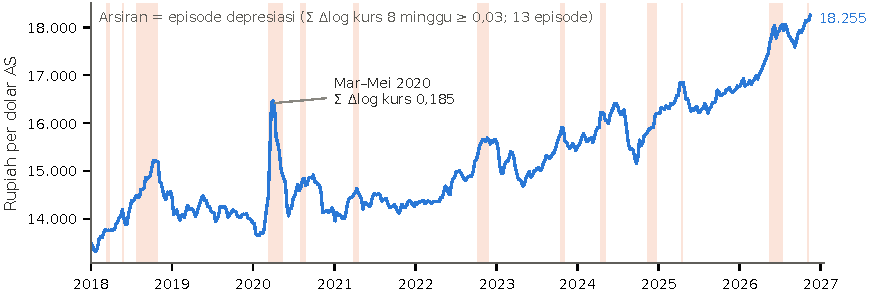
\includegraphics[width=\textwidth]{figures/kurs_episode.pdf}
\caption{Kurs JISDOR mingguan 2018–2026 (rerata harian, Rp per dolar AS) dan 13 episode depresiasi. Episode = minggu ketika
jumlah perubahan log kurs dalam 8 minggu terakhir mencapai 0,03 atau lebih, dengan pemicu berdekatan digabung. Sumber: artefak
\texttt{drivers\_weekly} dan \texttt{episodes}, dibangun dari JISDOR Bank Indonesia.}
\label{fig:kurs}
\end{figure}

Teori dan bukti empiris menyatakan bahwa penerusan kurs ke harga konsumen jarang penuh. Margin distribusi dan biaya lokal menyerap
sebagian besar perubahan harga impor \citep{burstein2003,campa2010}. Seberapa sering harga disesuaikan dan mata uang penagihan juga
menentukan besarnya penerusan \citep{gopinath2010,gopinath2020}. Untuk harga pangan di 17 negara berkembang, \citet{unuvar2026}
menemukan rerata penerusan kumulatif 0,213, dengan Indonesia terendah, yaitu $-0,012$ (galat baku 0,150; interval $-0,306$..$0,281$).
Studi lain yang mencakup Indonesia umumnya memakai inflasi agregat nasional
\citep{suarsih2016,widarjono2023,arintoko2024,ibrahim2025}.

Angka agregat yang mendekati nol bisa berarti tidak ada respons, tetapi bisa juga menyembunyikan respons yang saling meniadakan antar
komoditas atau antarprovinsi. Komoditas pangan terpapar kurs lewat jalur yang berbeda. Bawang putih, gula, dan daging sapi diimpor
langsung. Daging ayam dan telur bergantung pada pakan dari jagung dan bungkil kedelai yang harganya ditentukan pasar dunia. Harga
minyak goreng mengikuti paritas ekspor minyak sawit. Pasar provinsi juga berbeda dalam integrasi, struktur ekonomi, dan kebijakan
\citep{varela2013,aginta2022,persada2026}. Sementara itu, Bank Indonesia menerbitkan harga eceran harian per provinsi melalui PIHPS
\citep{bipihps2026}, sumber data yang kaya tetapi belum banyak dimanfaatkan untuk pertanyaan ini.

Tema lomba, \textit{Realizing Impactful Innovation through Creative and Sustainable Technology}, kami bingkai sebagai ketahanan
harga pangan. Target SDG 2.c meminta negara menjamin berfungsinya pasar komoditas pangan dan akses tepat waktu pada informasi pasar
untuk membatasi volatilitas harga pangan yang ekstrem \citep{un2015}. KAGAMI (dari bahasa Jepang \textit{kagami}, cermin)
memeriksa sejauh mana harga pangan eceran mencerminkan rupiah, lalu menyajikan hasilnya dalam bentuk yang dapat dipakai TPID.

\subsection{Rumusan masalah dan pertanyaan penelitian}

Pertanyaan pemandunya adalah apakah kepekaan harga pangan eceran terhadap rupiah lebih ditentukan oleh komoditasnya atau oleh
lokasinya. Pertanyaan ini kami pecah menjadi lima pertanyaan penelitian dan hipotesis yang dibekukan dalam praregistrasi
(Tabel~\ref{tab:rq}).

\begin{table}[!htbp]
\centering\small
\caption{Pertanyaan penelitian, hipotesis praregistrasi, dan jenis uji.}
\label{tab:rq}
\begin{tabularx}{\textwidth}{@{}l >{\RaggedRight}X l l@{}}
\toprule
Kode & Pertanyaan atau hipotesis & Uji utama & Jenis \\
\midrule
RQ1 & Besar dan kecepatan respons nasional per komoditas terhadap kurs dan harga dunia dalam rupiah & proyeksi lokal & deskriptif + MDE \\
RQ2 / H0-Het & Respons antarprovinsi pada $h=8$ lebih bervariasi daripada derau ($\tau^2>0$) untuk minimal satu komoditas & $Q$ vs plasebo, BH & konfirmatori \\
RQ2 & Provinsi membentuk kelompok kepekaan yang stabil & Ward vs plasebo & konfirmatori \\
RQ3 / H2 & Respons saat rupiah melemah berbeda dari saat menguat & Wald $\beta^{+}(8)=\beta^{-}(8)$ & konfirmatori bila MDE $\le 0,5$ \\
RQ4 / H3 & Provinsi yang lebih terpencil merespons lebih kecil pada $h=4$ & meta-regresi efek acak & konfirmatori \\
RQ4 / E1 & Komoditas impor langsung memiliki penerusan lebih besar & Kendall $\tau_b$ eksak & deskriptif \\
RQ5 / H5 & Fitur kurs menurunkan galat prediksi 8 minggu untuk jalur impor & rasio MAE + DM, Holm & konfirmatori \\
E2 & Respons berbeda antarperiode HET/HAP & proyeksi lokal per rezim & eksploratif \\
\bottomrule
\end{tabularx}
\end{table}

\subsection{Tujuan dan manfaat}

Penelitian ini bertujuan (1) mengukur profil respons nasional 10 komoditas terhadap kurs dan harga dunia dalam rupiah beserta
interval dan daya ujinya, (2) menguji apakah respons berbeda antarprovinsi dan apakah provinsi membentuk kelompok, terhadap
distribusi null yang eksplisit, (3) menguji asimetri antara pelemahan dan penguatan rupiah, (4) menelusuri karakteristik terukur
yang berasosiasi dengan perbedaan respons, dan (5) menilai apakah fitur kurs memperbaiki prediksi perubahan harga 4 dan 8 minggu.

Manfaatnya ada pada tiga kelompok pengguna. Bagi TPID, KAGAMI memberi batas atas kenaikan harga yang konsisten dengan pelemahan
rupiah dalam Rupiah per kilogram atau liter, profil respons per komoditas, dan profil per provinsi melalui aplikasi web. Bagi
peneliti, kami menyediakan dataset turunan yang terintegrasi dan terdokumentasi dengan datasheet \citep{gebru2021}, beserta
pipeline yang dapat dijalankan ulang. Bagi praktik data mining, proyek ini memberi contoh praregistrasi, penilaian clustering
terhadap null plasebo, dan pelaporan hasil nol sebagai batas atas.

\subsection{Batasan}

Hasil penelitian ini bersifat asosiasional dan tidak mengidentifikasi efek kausal. KAGAMI tidak meramal kurs dan tidak mengamati
rantai pasok, misalnya biaya pengadaan importir, mata uang penagihan, atau stok. Cakupannya 10 komoditas, 34 provinsi dalam
kerangka lama (provinsi pemekaran Papua digabung ke induknya), periode 2018-01-01 sampai pembekuan 2026-11-21, dan frekuensi
mingguan. Harga yang dipakai adalah harga pasar tradisional PIHPS untuk satu varian representatif per komoditas. Evaluasi prediktif
bersifat pseudo-real-time karena vintage revisi data tidak tersedia. Kebutuhan TPID belum divalidasi lewat wawancara, sehingga
KAGAMI kami posisikan sebagai prototipe riset untuk analitik pendukung keputusan.

% ===========================================================================================================
\section{Kajian Pustaka}

Kajian ini bersifat tematik, bukan tinjauan sistematis. Kami mengelompokkan rujukan ke dalam empat tema. Identitas setiap rujukan
kami cocokkan dengan DOI, arXiv, atau halaman resmi penerbitnya, dan klaim kuantitatif yang kami kutip dari studi lain kami cek pada
teks lengkapnya.

\subsection{Penerusan kurs dan sumber heterogenitasnya}

Penerusan kurs ke harga konsumen lebih kecil daripada ke harga impor. \citet{burstein2003} menunjukkan bahwa biaya distribusi lokal
mengisi porsi besar harga eceran, sehingga perubahan kurs teredam. \citet{campa2010} mengaitkan kepekaan indeks harga konsumen
terhadap kurs dengan margin distribusi, porsi input impor, dan paparan perdagangan. Di tingkat perusahaan, \citet{gopinath2010}
menemukan bahwa barang yang harganya lebih sering disesuaikan memiliki penerusan jangka panjang yang lebih tinggi, \citet{amiti2014}
mengaitkan penerusan yang tidak penuh dengan intensitas impor dan pangsa pasar eksportir, dan \citet{gopinath2020} menekankan peran
mata uang penagihan dolar. Heterogenitas penerusan juga terdokumentasi dengan data mikro di Thailand \citep{apaitan2024} dan
Meksiko \citep{solorzano2023}, serta dengan metode nonparametrik lintas negara \citep{kohlscheen2026}. Untuk harga pangan,
\citet{unuvar2026} menemukan penerusan yang lebih kuat ketika inflasi pangan tahunan melampaui 6,8–7,6\%, dengan estimasi Indonesia
yang paling rendah di antara 17 negara.

\subsection{Bukti Indonesia}

\citet{suarsih2016} mengukur dampak perubahan nilai tukar terhadap indeks harga konsumen bahan makanan. \citet{widarjono2023} mengkaji
asimetri penerusan kurs ke inflasi di beberapa negara ASEAN, \citet{arintoko2024} meneliti efek asimetris harga energi dan pangan
global serta dinamika kurs terhadap inflasi Indonesia, dan \citet{ibrahim2025} menelaah penerusan harga komoditas ke inflasi
Indonesia. Studi-studi ini bekerja pada inflasi agregat nasional. Di tingkat daerah, \citet{varela2013} meneliti integrasi pasar dan
transmisi harga antarwilayah beserta penentunya, \citet{aginta2022} menemukan bahwa efek kebijakan moneter berbeda antarprovinsi
sesuai struktur ekonominya, dan \citet{persada2026} menunjukkan bahwa harga beras di 26 provinsi pada 2018–2022 merespons instrumen
kebijakan secara berbeda di wilayah surplus dan defisit. Harga pembelian pemerintah hanya berasosiasi dengan harga eceran di provinsi
defisit, sedangkan stok cadangan beras pemerintah hanya berasosiasi dengan harga yang lebih rendah di provinsi surplus.

\subsection{Metode respons dinamis dan inferensi}

Proyeksi lokal \citep{jorda2005} memperkirakan respons pada setiap horizon dengan regresi terpisah, dan pada populasi menghasilkan
respons impuls yang sama dengan VAR \citep{plagborg2021}. Penambahan lag pada proyeksi lokal membuat inferensinya lebih tahan
terhadap persistensi \citep{montiel2021}. Ketika banyak unit mikro merespons guncangan agregat yang sama, informasi tentang guncangan
itu bertumpu pada dimensi waktu \citep{almuzara2024}. Hal ini menjadi dasar kami mengelompokkan galat baku per minggu. Pendekatan
hierarkis untuk proyeksi lokal pada deret pendek juga mulai berkembang \citep{clark2026}. Untuk ketidakpastian, kami memakai
bootstrap blok bergerak \citep{kunsch1989}, estimator heterogenitas $\tau^2$ \citep{dl1986}, koreksi galat baku berkelompok untuk
sampel kecil \citep{pustejovsky2018}, serta koreksi multiplisitas Benjamini–Hochberg dan Holm \citep{bh1995,holm1979}. Praregistrasi
memisahkan uji konfirmatori dari eksplorasi \citep{nosek2018}.

\subsection{Data mining harga pangan Indonesia}

Penelitian data mining harga pangan Indonesia yang kami temukan berfokus pada pengelompokan dan peramalan deret harga. \citet{rahkmawati2023}
mengelompokkan provinsi berdasarkan deret harga beras dengan jarak dynamic time warping. \citet{amatullah2025} membangun model peramalan
berbasis clustering untuk mengelompokkan provinsi menurut harga gula pasir. \citet{sumertajaya2024} mengembangkan model peramalan harga
komoditas pangan sebagai peringatan dini dengan clustering deret waktu multivariat, dan \citet{saputra2026} memakai model ensemble
boosting untuk meramal harga beras. Validitas clustering biasanya dinilai dengan indeks internal seperti silhouette
\citep{rousseeuw1987} dan stabilitas \citep{hennig2007}, sedangkan perbandingan akurasi ramalan memakai uji Diebold–Mariano
\citep{dm1995} dengan koreksi sampel kecil \citep{hln1997}. Model yang kami pakai untuk peramalan meliputi ridge \citep{hoerl1970},
gradient boosting \citep{friedman2001,pedregosa2011}, serta model deep learning dan foundation model deret waktu
\citep{nie2023,chen2023,das2024}. Proses eksplorasi pasca-praregistrasi kami mengikuti tahapan CRISP-DM \citep{schroer2021}.

\subsection{Celah penelitian}

Sejauh penelusuran kami, belum ada studi yang mengukur respons harga eceran mingguan per komoditas dan per provinsi di Indonesia
terhadap kurs sekaligus harga dunia dalam rupiah, lalu menilai struktur regional dan nilai prediktifnya terhadap distribusi null
yang eksplisit. Studi terdekat adalah \citet{unuvar2026} untuk penerusan kurs ke inflasi pangan tingkat negara dan
\citet{persada2026} untuk heterogenitas harga beras antarprovinsi.

% ===========================================================================================================
\section{Solusi Usulan}

\subsection{Deskripsi solusi}

KAGAMI adalah pipeline data mining yang berjalan dari data mentah sampai aplikasi (Gambar~\ref{fig:pipeline}). Tahap 0 membangun
dataset turunan. Task 1 mengukur profil respons, Task 2 mencari pola regional, Task 3 menguji asosiasi dan asimetri, dan Task 4
menilai nilai prediktif. Ketahanan hasil diuji dengan serangkaian pemeriksaan wajib dan opsional. Setiap tahap menulis artefak
dengan kontrak kolom yang diperiksa otomatis (39 artefak), dan setiap eksekusi dicatat dengan sidik jari sha256 input dan
outputnya. Kode ditulis dalam Python. Mesin statistiknya kami tulis sendiri dengan NumPy dan SciPy, dan model prediksinya memakai
scikit-learn \citep{pedregosa2011}. Hipotesis, varian komoditas, dan parameter dibekukan di gerbang praregistrasi (G6) pada
20 November 2026 pukul 23.29 WIB, sebelum respons Task 1 dilihat.

\begin{figure}[!tbp]
\centering
\begin{tikzpicture}[
  box/.style={draw=kgblue!70, fill=kgblue!5, rounded corners=2pt, align=left, font=\footnotesize, inner sep=4pt,
              text width=#1},
  gate/.style={draw=kgorange, fill=kgorange!8, rounded corners=2pt, align=center, font=\footnotesize, inner sep=3.5pt,
               text width=15.3cm},
  arr/.style={-{Stealth[length=2.2mm]}, semithick, color=kggray},
  node distance=4.5mm]
\node[box=15.3cm] (src) {\textbf{Sumber data.} PIHPS eceran harian (Bank Indonesia) \textperiodcentered{} JISDOR \textperiodcentered{}
  Pink Sheet (Bank Dunia) \textperiodcentered{} Brent dan indeks dolar (FRED) \textperiodcentered{} FAOSTAT \textperiodcentered{}
  impor BPS dan UN Comtrade \textperiodcentered{} Panel Harga Bapanas \textperiodcentered{} riwayat HET/HAP (tabel tim dari dokumen hukum)};
\node[box=15.3cm, below=of src] (s0) {\textbf{Tahap 0: dataset turunan.} Panel mingguan 34 provinsi $\times$ 10 komoditas dengan
  status sel, kelayakan seri, penggerak mingguan, harga dunia dalam rupiah dengan tanggal ketersediaan, 13 episode depresiasi,
  panel 7 wilayah, tabel tim (konkordansi, rasio impor, regulasi, fitur provinsi), MDE, dan laporan kualitas data};
\node[gate, below=of s0] (g6) {\textbf{Praregistrasi G6 (20 Nov 2026).} Hipotesis, varian, bobot pakan, dan parameter dibekukan
  sebelum respons dilihat};
\node[box=3.26cm, below=7mm of g6.south west, anchor=north west] (t1) {\textbf{Task 1.} Proyeksi lokal nasional, studi peristiwa,
  deviasi provinsi, bootstrap blok, 499 plasebo};
\node[box=3.26cm, right=4mm of t1.north east, anchor=north west] (t2) {\textbf{Task 2.} Heterogenitas vs plasebo, clustering
  Ward, stabilitas, struktur tertanam};
\node[box=3.26cm, right=4mm of t2.north east, anchor=north west] (t3) {\textbf{Task 3.} Kendall eksak, meta-regresi, asimetri,
  rezim HET/HAP, kalibrasi plasebo};
\node[box=3.26cm, right=4mm of t3.north east, anchor=north west] (t4) {\textbf{Task 4.} Rolling-origin as-of, model M0–M3,
  uji DM, ablation kurs};
\node[box=15.3cm, anchor=north] (rb) at ([yshift=-9mm]current bounding box.south -| s0) {\textbf{Ketahanan dan validasi.} Tier 1: lag, horizon,
  sub-periode, tanpa Mar–Jun 2020, dekomposisi kurs, frekuensi bulanan. Tier 2: varian lain, observasi terakhir, Panel Harga
  Bapanas. Validasi V2 (2026) dan V4 (proyeksi lokal vs studi peristiwa)};
\node[box=15.3cm, below=of rb] (out) {\textbf{Keluaran.} 39 artefak berkontrak dan log eksekusi $\rightarrow$ aplikasi Streamlit
  (8 halaman hasil, 2 lampiran), paket juri dengan reproduksi tiga tingkat, temuan, dan makalah ini};
\draw[arr] (src) -- (s0);
\draw[arr] (s0) -- (g6);
\foreach \t in {t1,t2,t3,t4} {\draw[arr] (g6.south) ++(0,0) |- ($(g6.south)!0.5!(g6.south |- \t.north)$) -| (\t.north);}
\foreach \t in {t1,t2,t3,t4} {\draw[arr] (\t.south) |- ($(\t.south |- rb.north)+(0,5.5mm)$) -| (rb.north);}
\draw[arr] (t1.east) -- (t1.east -| t2.west);
\draw[arr] (rb) -- (out);
\end{tikzpicture}
\caption{Alur KAGAMI. Task 2 dan Task 3 memakai keluaran Task 1, sedangkan Task 4 berjalan paralel. Semua tahap membaca dan
menulis artefak dengan kontrak kolom yang dites otomatis.}
\label{fig:pipeline}
\end{figure}

\subsection{Dataset}

\subsubsection{Sumber data}
Tabel~\ref{tab:sumber} merangkum sumber utama. Outcome adalah harga eceran harian PIHPS di 34 provinsi untuk 10 komoditas
\citep{bipihps2026}. Penggerak pertama adalah kurs JISDOR \citep{bijisdor2026}. Penggerak kedua adalah harga dunia padanan dari
Pink Sheet \citep{worldbank2026} yang dikonversi ke rupiah. Brent dan indeks dolar dari FRED \citep{fred2026} masing-masing menjadi
kontrol dan bahan dekomposisi kurs. Rasio impor dihitung dari FAOSTAT \citep{fao2026}, impor BPS \citep{bps2026}, dan UN Comtrade,
dan Panel Harga Pangan Bapanas \citep{bapanas2026} menjadi outcome pembanding. Riwayat HET/HAP disusun tim dari dokumen hukum
publik, dengan status verifikasi untuk setiap tanggal.

\begin{table}[!htbp]
\centering\small
\caption{Sumber data utama. Data mentah tanpa hak redistribusi tidak ikut paket proyek. Yang dikirim adalah turunannya, atas izin
Bank Indonesia untuk data turunan PIHPS.}
\label{tab:sumber}
\begin{tabularx}{\textwidth}{@{}>{\RaggedRight}p{3.9cm} >{\RaggedRight}X >{\RaggedRight}p{3.7cm} l@{}}
\toprule
Sumber & Frekuensi dan cakupan & Peran & Dikirim mentah \\
\midrule
PIHPS (Bank Indonesia) & harian, 34 provinsi, 2017-03-28..2026-11-19 & outcome harga eceran & tidak \\
JISDOR (Bank Indonesia) & harian, 2013-05-20..2026-11-18 & penggerak kurs & tidak \\
Pink Sheet (Bank Dunia) & bulanan, sampai 2026-10 & harga dunia padanan & ya (CC BY 4.0) \\
FRED: Brent, indeks dolar & harian & kontrol, dekomposisi kurs & ya \\
FAOSTAT SUA & tahunan 2010–2023 & rasio impor & ya (CC BY 4.0) \\
Impor BPS (HS8), UN Comtrade & bulanan 2017–2026 & rasio impor bawang putih, cek silang & tidak \\
Panel Harga Bapanas & bulanan, 2022-01..2026-10 & outcome pembanding & tidak \\
Regulasi HET/HAP (tabel tim) & per tanggal penetapan & rezim kebijakan (E2) & ya \\
Jarak ke hub, kota sampel PIHPS & statis & fitur provinsi & ya \\
\bottomrule
\end{tabularx}
\end{table}

\subsubsection{Dataset turunan}
Harga mingguan setiap seri provinsi $\times$ komoditas adalah rerata harga hari kerja yang teramati dalam minggu ISO, diberi label
hari Senin. Hasilnya 157.760 sel, yaitu 34 provinsi $\times$ 10 komoditas $\times$ 464 minggu dari 2018-01-01 sampai 2026-11-16.
Setiap sel diberi status. Sebanyak 49,2\% sel teramati biasa, 49,2\% berupa rangkaian harga identik (minggu yang mayoritas hari
teramatinya termasuk rangkaian harga sama selama 5 hari atau lebih), 0,6\% minggu pendek, dan 1,0\% kosong. Rangkaian harga identik
terkonsentrasi pada komoditas yang harganya diatur: beras 92\%, daging sapi 90\%, minyak goreng 87\%, dan gula 85\%. Status ini
tidak membedakan harga yang memang tetap dari harga hari sebelumnya yang dipakai sumber ketika pasar tutup, sehingga kami tidak
memakainya untuk menyaring data. Sebanyak 337 dari 340 seri lolos aturan kelayakan (data kosong paling banyak 20\%, celah paling
lama 8 minggu, dan setiap tahun terisi minimal 70\%). Tiga seri cabai rawit (Aceh, Sumatra Barat, Kepulauan Riau) tidak layak.

Dataset turunan juga memuat penggerak mingguan, harga dunia padanan dalam rupiah untuk enam komoditas beserta tanggal
ketersediaannya, daftar 13 episode depresiasi (61 minggu, terbesar Maret–Mei 2020 dengan jumlah perubahan log kurs 0,185), panel
indeks 7 wilayah, dan tabel buatan tim. Tabel tim meliputi konkordansi PIHPS–HS–Pink Sheet–FAOSTAT, rasio impor langsung (bawang
putih 0,93, gula 0,37, daging sapi 0,29, bawang merah 0,069, beras 0,033, komoditas lain mendekati nol), riwayat HET/HAP, dan fitur
provinsi berupa jarak garis lurus ibu kota ke hub logistik terdekat (Jakarta, Surabaya, atau Makassar), kecukupan produksi beras,
dan jumlah kota sampel PIHPS. Semuanya memakai kunci yang sama (minggu, provinsi, komoditas). Kebaruan dataset ini ada pada integrasi
dan pengayaannya, terutama status sel, tanggal ketersediaan, dan regulasi bertanggal. Rinciannya kami dokumentasikan dalam bentuk
datasheet \citep{gebru2021}. Varian representatif dan padanan harga dunia setiap komoditas tercantum pada Tabel~\ref{tab:komoditas}.

\begin{table}[!htbp]
\centering\small
\caption{Komoditas, varian PIHPS representatif, jalur eksposur, dan padanan harga dunia.}
\label{tab:komoditas}
\begin{tabularx}{\textwidth}{@{}l X l l@{}}
\toprule
Komoditas & Varian representatif & Jalur eksposur & Padanan Pink Sheet \\
\midrule
Beras & Beras Kualitas Medium I & impor langsung & Rice, Thai 5\% \\
Bawang putih & Bawang Putih Ukuran Sedang & impor langsung & -- \\
Gula pasir & Gula Pasir Lokal & impor langsung & Sugar, world \\
Daging sapi & Daging Sapi Kualitas 1 & impor langsung & Beef \\
Daging ayam & Daging Ayam Ras Segar & input impor (pakan) & 0,6 jagung + 0,4 bungkil kedelai \\
Telur ayam & Telur Ayam Ras Segar & input impor (pakan) & 0,6 jagung + 0,4 bungkil kedelai \\
Minyak goreng & Minyak Goreng Kemasan Bermerk 1 & paritas ekspor & Palm oil \\
Bawang merah & Bawang Merah Ukuran Sedang & domestik & -- \\
Cabai merah & Cabai Merah Keriting & domestik & -- \\
Cabai rawit & Cabai Rawit Merah & domestik & -- \\
\bottomrule
\end{tabularx}
\end{table}

\subsection{Metode}

\subsubsection{Penggerak dan episode}
Penggerak kurs $e_t$ adalah rerata log JISDOR harian dalam minggu $t$, dengan perubahan $\Delta e_t$. Minggu tanpa fixing (cuti
Lebaran) meneruskan level minggu sebelumnya. Harga dunia dalam rupiah $w_{i,t}$ adalah log harga Pink Sheet padanan ditambah rerata
log JISDOR bulan yang sama. Karena harga dunia bulanan, $\Delta w_{i,t}$ hanya berubah pada minggu pertama setiap bulan, sehingga
tidak kolinear dengan $\Delta e_t$. Selama 2018–2026 simpangan baku $\Delta e_t$ adalah 0,0082, dengan 259 minggu depresiasi dan 200
minggu apresiasi. Episode depresiasi dimulai ketika jumlah $\Delta e$ dalam 8 minggu mencapai 0,03.

\subsubsection{Proyeksi lokal}
Untuk komoditas $i$, provinsi $r$, minggu $t$, dan horizon $h = 0,\dots,12$, kami mengestimasi
\begin{equation}
\begin{aligned}
y^{(h)}_{i,r,t} = {} & \alpha_{i,r,h} + \beta_{i,h}\,\Delta e_t + \omega_{i,h}\,\Delta w_{i,t}
+ \sum_{l=1}^{4}\left(\phi_{l}\,\Delta p_{i,r,t-l} + \psi_{l}\,\Delta e_{t-l} + \chi_{l}\,\Delta w_{i,t-l}\right) \\
& + \sum_{l=0}^{4}\pi_{l}\,\Delta b_{t-l} + S_{i,h}(t) + u_{i,r,t+h},
\end{aligned}
\label{eq:lp}
\end{equation}
dengan $y^{(h)}_{i,r,t} = p_{i,r,t+h} - p_{i,r,t-1}$ perubahan kumulatif log harga, $\alpha$ efek tetap seri, $\Delta b$
perubahan log Brent, dan $S(t)$ dummy bulan serta dummy minggu $-6$ sampai $+4$ di sekitar Idulfitri. Koefisien $\beta_{i,h}$ kira-kira
sama dengan persen perubahan harga eceran untuk setiap 1\% pelemahan rupiah. Galat baku dikelompokkan per minggu karena seluruh
informasi tentang kurs bervariasi menurut waktu. Penerusan kurs dihitung sebagai $PT(h) = \beta(h)/\gamma(h)$, dengan $\gamma(h)$
respons kurs terhadap dirinya sendiri ($\gamma(4)=1,44$, $\gamma(8)=1,32$, $\gamma(12)=1,03$). Untuk H2, $\beta\,\Delta e$ diganti
$\beta^{+}\Delta e^{+} + \beta^{-}\Delta e^{-}$, lalu kesamaan $\beta^{+}(8)=\beta^{-}(8)$ diuji dengan Wald.

\subsubsection{Inferensi, daya uji, dan studi peristiwa}
Ketidakpastian diukur dengan tiga cara. Pertama, galat baku berkelompok per minggu. Kedua, bootstrap blok bergerak 13 minggu dengan
499 replikasi (199 untuk komoditas non-fokus), yang memakai satu vektor indeks minggu per replikasi untuk harga dan penggerak semua
seri sehingga korelasi antarprovinsi dan antarkomoditas terjaga. Ketiga, 499 plasebo geser-melingkar yang menggeser $\Delta e$ dan
$\Delta w$ minimal 52 minggu terhadap harga. Plasebo ini mempertahankan struktur deret harga tetapi memutus kaitan waktunya dengan
penggerak. Interval resmi praregistrasi adalah yang lebih lebar antara $\pm 1,96\cdot SE$ dan persentil bootstrap. Respons yang
intervalnya memuat nol kami sebut tidak terdeteksi dan kami laporkan sebagai batas atas.

Sebelum melihat $\beta$, kami menghitung efek terkecil yang dapat dideteksi, $\mathrm{MDE} = 2,80\cdot SE$ (taraf nyata 5\%, daya
80\%). Gerbang G-power menyatakan bahwa bila MDE untuk $PT(8)$ melebihi 0,5 pada bawang putih, gula, dan minyak goreng sekaligus,
proyeksi lokal turun menjadi analisis sekunder. Studi peristiwa membandingkan perubahan harga dari minggu sebelum episode sampai
$h$ minggu sesudahnya dengan 499 jendela plasebo yang berawal di luar episode.

\subsubsection{Heterogenitas provinsi dan pola regional}
Deviasi provinsi $\delta_{i,r,h}$ diperoleh dari spesifikasi (\ref{eq:lp}) pada log harga yang dikurangi rerata lintas provinsi,
sehingga guncangan nasional terhapus dan $\sum_r \delta_{i,r,h} = 0$. Untuk setiap komoditas pada $h=8$ kami menghitung statistik
$Q$, $\tau^2$ DerSimonian–Laird (REML sebagai cek), dan $I^2$, lalu membandingkannya dengan distribusi yang sama dari 499 replikasi
plasebo. H0-Het ditolak bila $q$ Benjamini–Hochberg atas 10 komoditas paling besar 0,05. Deviasi disusutkan dengan empirical Bayes,
$\hat\delta^{EB} = \mu + \tau^2/(\tau^2+s^2)\,(\delta-\mu)$, sehingga $\tau^2 = 0$ menyusutkan semua provinsi ke rerata.

Clustering memakai matriks 34 provinsi $\times$ fitur respons tersusut (respons kurs dan harga dunia komoditas fokus pada $h$ = 4, 8,
12) yang distandardisasi, dengan metode Ward \citep{ward1963}. Untuk $k = 2,\dots,6$ kami mencatat silhouette maksimum
\citep{rousseeuw1987}. Struktur diterima hanya bila nilai itu melebihi persentil 95 silhouette maksimum dari matriks plasebo yang
diproses identik. Bila tidak, $k = 1$. Stabilitas dinilai dengan kesesuaian terhadap K-Means melalui adjusted Rand index
\citep{hubert1985} dan dengan Jaccard bootstrap \citep{hennig2007}. Untuk mengetahui apa yang mampu dideteksi desain ini, kami menanam struktur buatan berupa 2 atau 3 kelompok acak
dengan selisih respons $\delta$ = 0,1–0,5 (RMS per fitur) pada deviasi plasebo mentah, memprosesnya persis seperti data asli, dan
mencatat peluang struktur itu ditemukan kembali (200 replikasi per sel). Batas deteksi adalah $\delta$ terkecil dengan peluang
minimal 0,8.

\subsubsection{Asosiasi, asimetri, dan rezim kebijakan}
Di tingkat komoditas, korelasi peringkat Kendall $\tau_b$ antara $PT(8)$ dan rasio impor langsung diuji dengan permutasi eksak atas
$10! = 3.628.800$ urutan. Di tingkat provinsi, meta-regresi efek acak menghubungkan $\delta_{i,r,h}$ dengan paling banyak tiga
fitur provinsi, yaitu $\ln(1+\text{jarak ke hub})$, kecukupan produksi beras, dan jumlah kota sampel. Intervalnya adalah yang lebih
lebar antara CR2 \citep{pustejovsky2018} dan bootstrap. H3 menguji koefisien jarak pada $h=4$ secara satu arah. Eksplorasi E2
mengestimasi spesifikasi (\ref{eq:lp}) per rezim di antara tanggal penetapan HET/HAP yang terverifikasi, dengan interval yang
dikalibrasi plasebo.

\subsubsection{Evaluasi prediktif}
Task 4 memprediksi $p_{t+h} - p_t$ untuk $h$ = 4 dan 8 minggu. Origin dibuat setiap 4 minggu sejak 2021-01-04, menghasilkan
76 origin untuk $h=4$ dan 75 untuk $h=8$. Model hanya dilatih pada baris yang targetnya sudah terealisasi sebelum origin, dan harga
dunia hanya dipakai sesudah tanggal ketersediaannya (hari kerja ke-2 bulan berikutnya). M0 memprediksi tanpa perubahan. M1 adalah
regresi ridge \citep{hoerl1970} dengan lag perubahan harga, bulan, Idulfitri, dan Brent. M2 menambahkan perubahan kurs dan harga
dunia 1, 4, dan 8 minggu serta penanda episode yang dihitung real-time. M3 adalah gradient boosting dengan fitur M2 ditambah
identitas komoditas dan wilayah. Akurasi dibandingkan dengan MAE, RMSE, rasio terhadap M1, dan uji Diebold–Mariano dengan varians
HAC dan koreksi HLN. Kami selalu melaporkan arah statistik DM. H5 menguji M2 pada $h=8$ untuk origin dengan pergerakan kurs besar
(perubahan 4 minggu di atas persentil 80 data latih), pada jalur impor langsung dan input impor, dengan koreksi Holm atas dua jalur.

\subsubsection{Ketahanan dan tingkat bukti}
Tier 1 wajib mengulang estimasi dengan lag 2, 4, dan 8; $h$ 8 dibanding 12; sub-periode sebelum dan sesudah perubahan metode JISDOR
(2021-04-05); tanpa Maret–Juni 2020 dan bulan Brent ekstrem; dekomposisi $\Delta e$ menjadi komponen dolar global dan komponen
spesifik rupiah; serta frekuensi bulanan. Tier 2 memakai varian PIHPS lain, harga observasi terakhir, definisi keterpencilan lain,
dan Panel Harga Bapanas. Validasi V4 membandingkan implikasi proyeksi lokal dengan studi peristiwa.

Setiap angka di makalah ini termasuk salah satu dari tiga tingkat bukti. Tingkat 1 adalah uji praregistrasi dengan interval resmi.
Tingkat 2 adalah interval terkalibrasi plasebo yang kami tambahkan sesudah G6, setelah menemukan masalah inferensi yang dijelaskan
pada Bagian~\ref{sec:inferensi}. Tingkat 3 adalah eksplorasi Task 4 sesudah praregistrasi, yang tidak menguji hipotesis. Dua deviasi
praregistrasi kami catat terbuka: item FAOSTAT beras diganti beras giling dan patah karena item ``Rice'' ternyata gabah, dan dua kunci
konfigurasi ditambahkan sesudah G6.

\subsection{Perbedaan dengan solusi sebelumnya}

Tabel~\ref{tab:beda} membandingkan KAGAMI dengan dua kelompok studi terdekat. Studi penerusan kurs bekerja pada inflasi agregat,
sedangkan studi data mining harga pangan Indonesia yang kami temukan berfokus pada pengelompokan dan peramalan deret harga. KAGAMI berfokus pada kaitan
harga dengan kurs dan harga dunia di tingkat komoditas dan provinsi, dengan null eksplisit untuk setiap klaim pola.

\begin{table}[!htbp]
\centering\small
\caption{Perbedaan KAGAMI dengan studi terdekat. Dua kolom pembanding meringkas fokus utama studi yang dikutip, bukan menilai
kualitasnya.}
\label{tab:beda}
\begin{tabularx}{\textwidth}{@{}>{\RaggedRight}p{2.6cm} >{\RaggedRight}X >{\RaggedRight}X >{\RaggedRight}X@{}}
\toprule
Aspek & Penerusan kurs agregat \citep{suarsih2016,widarjono2023,unuvar2026} & Data mining harga pangan Indonesia \citep{rahkmawati2023,sumertajaya2024,amatullah2025,saputra2026} & KAGAMI \\
\midrule
Unit analisis & negara atau nasional, bulanan & provinsi, satu atau beberapa komoditas & 10 komoditas $\times$ 34 provinsi, mingguan \\
Kaitan dengan kurs & kurs terhadap indeks harga & fokus pada deret harga & kurs dan harga dunia padanan dalam rupiah, dengan kontrol Brent dan musim \\
Pola regional & -- & pengelompokan provinsi menurut deret harga & kelompok respons dinilai terhadap 499 plasebo, batas deteksi dari struktur tertanam \\
Inferensi & galat baku model & ukuran akurasi atau validitas internal & galat baku per minggu, bootstrap blok, plasebo, uji ukuran kalibrasi \\
Evaluasi prediktif & -- & akurasi peramalan & rolling-origin as-of, uji DM berarah, ablation fitur kurs \\
Praregistrasi & -- & -- & hipotesis dibekukan sebelum respons dilihat \\
Produk & makalah & model peramalan & aplikasi web, batas atas dalam Rupiah, paket reproduksi tiga tingkat \\
\bottomrule
\end{tabularx}
\end{table}

\subsection{Matriks evaluasi}

Tabel~\ref{tab:evaluasi} merangkum metrik, acuan, dan aturan keputusan setiap pertanyaan. Untuk uji praregistrasi, aturan ini
ditetapkan sebelum hasil dilihat. Untuk eksplorasi, kriterianya ditulis sebelum setiap pengukuran.

\begin{table}[!htbp]
\centering\small
\caption{Matriks evaluasi. Interval selalu 95\%.}
\label{tab:evaluasi}
\begin{tabularx}{\textwidth}{@{}>{\RaggedRight}p{2.5cm} >{\RaggedRight}X >{\RaggedRight}p{3.4cm} >{\RaggedRight}X@{}}
\toprule
Pertanyaan & Metrik & Acuan atau null & Aturan keputusan \\
\midrule
RQ1 respons & $\beta_e(h)$, $\omega(h)$, $PT(h)$ dengan interval resmi; MDE & nol & terdeteksi bila interval tidak memuat nol; selain itu batas atas \\
RQ2 heterogenitas & $Q$, $\tau^2$, $I^2$, $\bar\rho$; $p$ plasebo & 499 plasebo & H0-Het ditolak bila $q$ BH $\le 0,05$ \\
RQ2 kelompok & silhouette maksimum, ARI, Jaccard & persentil 95 plasebo; Jaccard 0,6 & $k>1$ hanya bila silhouette melampaui acuan \\
Batas deteksi & peluang ditemukan kembali & 0,8 & $\delta$ terkecil yang mencapai 0,8 \\
RQ3 asimetri & $\beta^{+}(8)-\beta^{-}(8)$, $p$ Wald & nol; MDE asimetri & konfirmatori hanya bila MDE asimetri $PT(8) \le 0,5$ \\
RQ4 asosiasi & Kendall $\tau_b$, $p$ eksak; koefisien meta-regresi & nol & H3 didukung bila koefisien $h=4$ negatif dengan $p$ satu sisi $<0,05$ \\
RQ5 prediksi & MAE, RMSE, rasio terhadap M1, DM (dengan arah) & M1; rasio 1 & H5 didukung bila $p$ Holm $<0,05$ untuk M2 lebih akurat \\
Ketahanan & sel cocok, kesamaan tanda & estimasi utama & dilaporkan per cek \\
Eksplorasi Task 4 & F1 makro, presisi daftar pantau, average precision & tebakan mayoritas, aturan naif, laju-dasar & interval bootstrap blok origin; koreksi BH atau Holm \\
\bottomrule
\end{tabularx}
\end{table}

% ===========================================================================================================
\section{Hasil Eksperimen dan Pengujian}

\subsection{Daya uji}

MDE untuk $PT(8)$ adalah 2,52 untuk bawang putih, 0,90 untuk gula, dan 0,465 untuk minyak goreng. Karena minyak goreng berada di
bawah 0,5, proyeksi lokal tetap menjadi analisis utama. MDE asimetri $PT(8)$ hanya memenuhi syarat konfirmatori untuk beras (0,44)
dan daging sapi (0,32), sehingga H2 bersifat konfirmatori untuk dua komoditas itu dan deskriptif untuk delapan lainnya (MDE 1,0–9,3).

\subsection{RQ1: respons nasional per komoditas}

Tabel~\ref{tab:rq1} dan Gambar~\ref{fig:respons} menunjukkan bahwa respons nasional terhadap kurs sebagian besar tidak terdeteksi.
Pada $h=8$ semua interval resmi respons kurs memuat nol. Untuk beras, penerusan $PT(8)$ di atas 0,11 dapat dikesampingkan, dan untuk
daging sapi di atas 0,13. Untuk cabai dan bawang, interval sangat lebar (MDE $PT(8)$ 1,84–3,75), sehingga hasil nolnya hampir tidak
informatif.

\begin{table}[!htbp]
\centering\small
\caption{Respons nasional pada $h = 8$ dengan interval resmi. Satuan: perubahan log harga per 1 perubahan log penggerak, kira-kira
persen per 1\%. Sumber: artefak \texttt{profiles}.}
\label{tab:rq1}
\begin{tabular}{@{}l l c c c@{}}
\toprule
Komoditas & Jalur & $\beta_e(8)$ & $PT(8)$ & $\omega(8)$ \\
\midrule
Beras & impor langsung & 0,01 \ci{−0,25}{0,18} & 0,00 \ci{−0,21}{0,11} & 0,06 \ci{−0,03}{0,14} \\
Bawang putih & impor langsung & −0,68 \ci{−2,93}{2,41} & −0,51 \ci{−1,77}{1,55} & -- \\
Gula pasir & impor langsung & 0,66 \ci{−0,27}{1,44} & 0,50 \ci{−0,25}{0,93} & −0,00 \ci{−0,26}{0,21} \\
Daging sapi & impor langsung & 0,02 \ci{−0,14}{0,17} & 0,01 \ci{−0,12}{0,13} & −0,00 \ci{−0,05}{0,08} \\
Daging ayam & input impor & −1,67 \ci{−2,61}{0,05} & −1,27 \ci{−1,78}{0,05} & −0,26 \ci{−0,55}{0,36} \\
Telur ayam & input impor & −0,53 \ci{−1,21}{0,49} & −0,40 \ci{−0,99}{0,37} & −0,22 \ci{−0,40}{0,26} \\
Minyak goreng & paritas ekspor & −0,23 \ci{−0,58}{0,38} & −0,17 \ci{−0,50}{0,29} & 0,21 \ci{−0,01}{0,36} \\
Bawang merah & domestik & −0,81 \ci{−2,52}{2,66} & −0,62 \ci{−1,93}{2,31} & -- \\
Cabai merah & domestik & 1,37 \ci{−2,91}{4,63} & 1,04 \ci{−2,21}{3,55} & -- \\
Cabai rawit & domestik & 0,76 \ci{−4,83}{4,14} & 0,57 \ci{−4,18}{3,06} & -- \\
\bottomrule
\end{tabular}
\end{table}

\begin{figure}[!tbp]
\centering
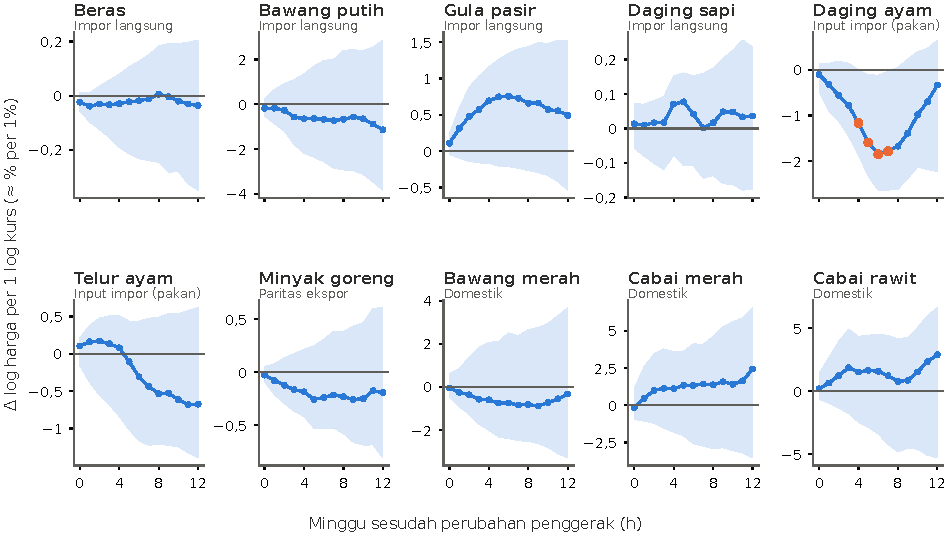
\includegraphics[width=\textwidth]{figures/respons_kurs.pdf}
\caption{Respons kumulatif nasional harga eceran terhadap kurs, $\beta_e(h)$, untuk $h = 0..12$ minggu. Pita = interval 95\%
resmi. Titik oranye = horizon yang intervalnya tidak memuat nol. Skala sumbu tegak berbeda antarpanel. Asosiasi historis, bukan
hubungan sebab-akibat. Sumber: artefak \texttt{profiles}.}
\label{fig:respons}
\end{figure}

\begin{figure}[!tbp]
\centering
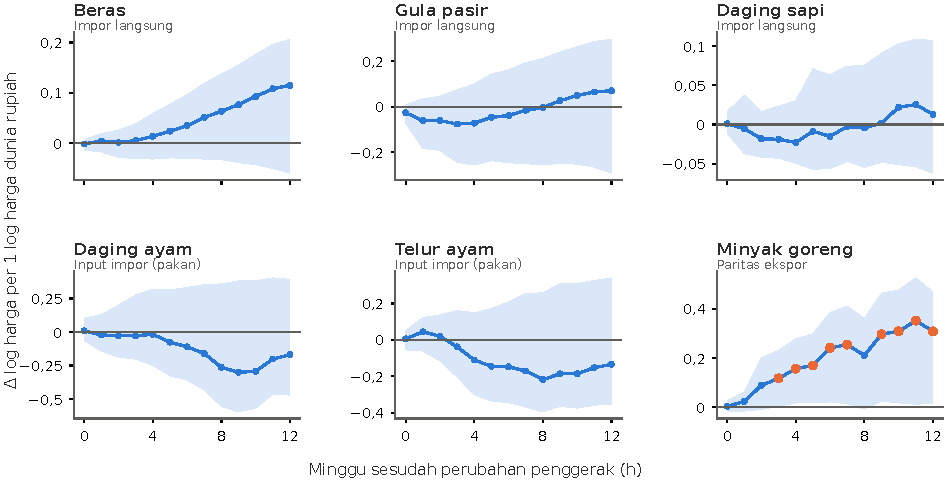
\includegraphics[width=0.92\textwidth]{figures/respons_dunia.pdf}
\caption{Respons kumulatif nasional terhadap harga dunia padanan dalam rupiah, $\omega(h)$, untuk enam komoditas yang memiliki
padanan Pink Sheet. Notasi sama dengan Gambar~\ref{fig:respons}. Sumber: artefak \texttt{profiles}.}
\label{fig:dunia}
\end{figure}

Asosiasi yang paling konsisten ada pada minyak goreng dan harga sawit dunia dalam rupiah (Gambar~\ref{fig:dunia}). Menurut interval resmi,
$\omega(4) = 0,16$ \ci{0,02}{0,28} dan $\omega(12) = 0,31$ \ci{0,02}{0,47}, sedangkan $\omega(8) = 0,21$ \ci{−0,01}{0,36} masih
memuat nol. Pada $h=8$ semua cek Tier 1 memberi interval di atas nol. Asosiasinya lebih kecil sebelum April 2021, yaitu 0,07
\ci{0,03}{0,10}, dibanding sesudahnya, 0,22 \ci{0,06}{0,37}.

Kenaikan kurs berasosiasi dengan penurunan harga daging ayam, arah yang berlawanan dengan dugaan jalur pakan impor. Interval resmi
$\beta_e(4) = -1,16$ \ci{−1,86}{−0,00} berbatas atas tepat di nol, dan $\beta_e(8) = -1,67$ \ci{−2,61}{0,05} memuat nol. Asosiasi ini
tidak tahan semua pemeriksaan. Tanpa Maret–Juni 2020 dan bulan Brent ekstrem estimasinya menjadi $-0,96$ \ci{−2,05}{0,14}, dan pada
frekuensi bulanan $-0,60$ \ci{−1,33}{0,13}. Komponen kurs yang spesifik rupiah memberi $-1,89$ \ci{−3,02}{−0,76}, sehingga asosiasinya
tidak semata mengikuti pergerakan dolar global. Estimasi gula $\beta_e(4) = 0,69$ lolos kalibrasi plasebo, tetapi berubah menjadi
$-0,03$ tanpa Maret–Juni 2020 dan sesudah April 2021, sehingga tidak kami tafsirkan sebagai temuan.

Studi peristiwa menghasilkan 390 sel nasional (13 episode $\times$ 10 komoditas $\times$ $h$ 4, 8, 12). Hanya 19 sel (4,9\%) yang
memiliki $p$ plasebo di bawah 0,05, setara dengan yang diharapkan dari kebetulan.

\subsection{RQ2: komoditas atau lokasi}

Tabel~\ref{tab:het} menunjukkan uji H0-Het. Heterogenitas antarprovinsi di atas plasebo terdeteksi pada telur ayam ($q$ 0,040) dan
daging ayam ($q$ 0,050). Penolakan daging ayam berada tepat di ambang. Lima dari 499 plasebo melampaui $Q$ asli, dengan galat Monte
Carlo nilai $p$ sekitar 0,004, sehingga kami menyebutnya penolakan rapuh. Gula berada di dekat ambang ($q$ 0,067). Untuk bawang putih,
cabai rawit, daging sapi, dan minyak goreng $\tau^2 = 0$, sehingga semua provinsi disusutkan ke respons nasional. $\tau^2$ REML
sejalan: telur 0,283, daging ayam 0,676, gula 0,031, dan nol atau di bawah 0,001 untuk empat komoditas tersebut. Korelasi rata-rata
deviasi provinsi antarkomoditas $\bar\rho = 0,094$ ($p$ plasebo 0,198).

\begin{table}[!htbp]
\centering\small
\caption{Uji heterogenitas antarprovinsi (H0-Het) pada $h = 8$ terhadap kurs, 34 provinsi (cabai rawit 31). Sumber: artefak
\texttt{heterogeneity}.}
\label{tab:het}
\begin{tabular}{@{}l r r r r r@{}}
\toprule
Komoditas & $Q$ & $\tau^2$ & $I^2$ & $p$ plasebo & $q$ BH \\
\midrule
Telur ayam & 161,7 & 0,226 & 0,80 & 0,004 & 0,040 \\
Daging ayam & 132,6 & 0,456 & 0,75 & 0,010 & 0,050 \\
Gula pasir & 81,0 & 0,031 & 0,59 & 0,020 & 0,067 \\
Bawang merah & 92,5 & 0,592 & 0,64 & 0,095 & 0,238 \\
Cabai merah & 57,8 & 1,013 & 0,43 & 0,265 & 0,530 \\
Beras & 39,7 & 0,002 & 0,17 & 0,380 & 0,633 \\
Bawang putih, cabai rawit, daging sapi, minyak goreng & 18,5–31,3 & 0 & 0 & 0,64–0,98 & 0,92–0,98 \\
\bottomrule
\end{tabular}
\end{table}

Provinsi tidak membentuk kelompok. Silhouette Ward maksimum 0,184 (pada $k=3$) berada di bawah persentil 95 plasebo, 0,196, sehingga
$k = 1$ (Gambar~\ref{fig:regional}a). Uji struktur tertanam menunjukkan apa yang dapat dikesampingkan. Struktur 2 dan 3 kelompok
berukuran hampir sama dengan selisih respons 0,2 per fitur ditemukan kembali pada 99,5\% dan 96,5\% replikasi, sedangkan selisih 0,1
hanya pada 43\% dan 13\% (Gambar~\ref{fig:regional}b). Struktur berbentuk ini dengan selisih minimal 0,2 dapat dikesampingkan. Bentuk
lain, misalnya kelompok kecil, gradien geografis, atau perbedaan pada sebagian komoditas saja, belum diuji.

\begin{figure}[!tbp]
\centering
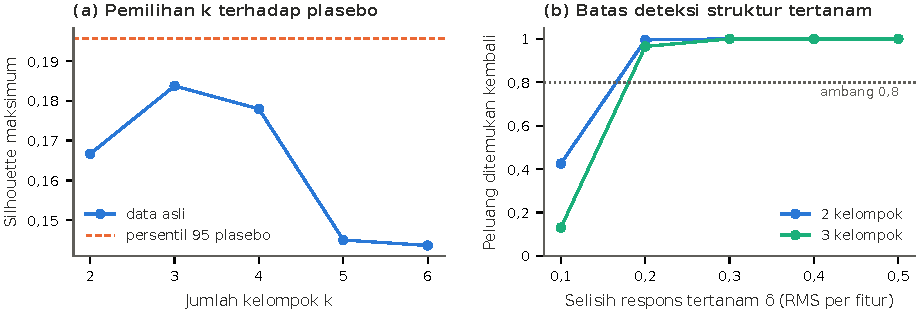
\includegraphics[width=\textwidth]{figures/struktur_regional.pdf}
\caption{(a) Silhouette maksimum clustering Ward per jumlah kelompok dibanding persentil 95 dari 499 plasebo. Tidak ada $k$ yang
melampaui acuan, sehingga $k = 1$. (b) Peluang struktur buatan 2 dan 3 kelompok ditemukan kembali menurut selisih respons yang
ditanam (200 replikasi per titik). Sumber: artefak \texttt{cluster\_selection} dan \texttt{planted\_recovery}.}
\label{fig:regional}
\end{figure}

Dengan interval terkalibrasi plasebo per provinsi dan koreksi BH atas seluruh 1.623 sel, tujuh deviasi provinsi bertahan, yaitu pada
daging ayam (Maluku, Papua, Kepulauan Riau), gula (Kalimantan Barat, Kalimantan Tengah), dan respons minyak goreng terhadap harga dunia
(Maluku Utara). Hasil ini deskriptif dan sejalan dengan uji heterogenitas.

\subsection{RQ3: pelemahan dibanding penguatan rupiah}

Kami tidak menemukan asimetri (Tabel~\ref{tab:h2}). Uji konfirmatori untuk beras dan daging sapi tidak menolak hipotesis nol.
Asimetri $PT(8)$ di atas 0,44 untuk beras dan di atas 0,32 untuk daging sapi akan terdeteksi dengan daya 80\%. Bawang putih memiliki
$p$ plasebo 0,022, tetapi nilai ini tidak bertahan koreksi atas 10 uji deskriptif, dan intervalnya memuat nol.

\begin{table}[!htbp]
\centering\small
\caption{Uji asimetri H2 pada $h=8$. Interval adalah gabungan interval Wald dan persentil bootstrap. Sumber: artefak
\texttt{asymmetry}.}
\label{tab:h2}
\begin{tabular}{@{}l l c c c@{}}
\toprule
Komoditas & Status & $\beta^{+}(8)-\beta^{-}(8)$ & $p$ Wald & $p$ plasebo \\
\midrule
Beras & konfirmatori & −0,14 \ci{−0,58}{0,47} & 0,49 & 0,62 \\
Daging sapi & konfirmatori & −0,26 \ci{−0,88}{0,21} & 0,089 & 0,28 \\
Bawang putih & deskriptif & −5,78 \ci{−10,23}{3,14} & 0,011 & 0,022 \\
7 komoditas lain & deskriptif & semua interval memuat nol & 0,11–0,87 & 0,16–0,88 \\
\bottomrule
\end{tabular}
\end{table}

\subsection{RQ4: karakteristik yang berasosiasi dengan respons}

Di antara 10 komoditas yang diamati, rasio impor langsung tidak berasosiasi monoton dengan $PT(8)$: Kendall $\tau_b = -0,045$
(jackknife $-0,65$..$0,56$), $p$ permutasi eksak 0,93. Mutu rasio impor tidak setara antarkomoditas. Bawang putih memakai impor BPS
dan Comtrade dengan produksi ATAP satu tahun karena FAOSTAT tidak memuat bawang putih kering, dan rasio ini tidak menangkap paparan
daging ayam dan telur lewat pakan.

Untuk H3, koefisien $\ln(1+\text{jarak ke hub})$ pada respons $h=4$, gabungan 10 komoditas dan 337 seri, adalah 0,007
\ci{−0,022}{0,033} per 1 simpangan baku jarak, dengan $p$ satu sisi 0,80. H3 tidak didukung, dan asosiasi negatif di atas 0,022 per
simpangan baku dapat dikesampingkan. Dari 88 koefisien meta-regresi eksploratif (jarak, kecukupan beras, dan jumlah kota sampel;
10 komoditas dan gabungannya; $h$ 4, 8, 12), tidak ada interval yang tidak memuat nol, dengan $q$ BH minimum 1,0. Sembilan koefisien
interaksi $\Delta e \times Z(r)$ dalam panel dengan efek tetap komoditas $\times$ minggu juga memuat nol, dengan yang terbesar pada
jarak ke hub untuk $h=8$: 0,16 \ci{−0,00}{0,33}.

\subsection{RQ5: nilai prediktif kurs}

Dalam evaluasi bersyarat pseudo-real-time pada 337 seri provinsi, fitur kurs dan harga dunia tidak menurunkan MAE
(Tabel~\ref{tab:task4}). M2 justru sedikit tetapi nyata kurang akurat dari M1 di kedua horizon, dengan statistik DM $-2,70$
($p$ dua sisi 0,009) dan $-2,29$ ($p$ 0,025). Untuk hipotesis bahwa M2 lebih akurat, $p$ satu sisi adalah 0,996 dan 0,987. Rasio
M2/M1 terburuk pada $h=8$ ada pada daging sapi (1,26), gula (1,10), dan beras (1,08), sedangkan cabai dan bawang merah berada di
sekitar 1 (Gambar~\ref{fig:prediksi}).

\begin{table}[!htbp]
\centering\small
\caption{Rasio MAE terhadap M1 pada semua origin. Rasio di atas 1 dan DM negatif berarti kurang akurat dari M1. Sumber: artefak
\texttt{forecast\_eval}.}
\label{tab:task4}
\begin{tabular}{@{}l c c@{}}
\toprule
Model & $h = 4$ (76 origin) & $h = 8$ (75 origin, 38 tidak tumpang tindih) \\
\midrule
M0, tanpa perubahan & 1,017 (DM $-1,90$; $p$ 0,062) & 1,016 (DM $-1,41$; $p$ 0,16) \\
M2, + kurs, harga dunia, episode & 1,009 (DM $-2,70$; $p$ 0,009) & 1,013 (DM $-2,29$; $p$ 0,025) \\
M3, gradient boosting + identitas & 1,037 (DM $-1,98$; $p$ 0,052) & 1,014 (DM $-0,63$; $p$ 0,53) \\
\bottomrule
\end{tabular}
\end{table}

\begin{figure}[!tbp]
\centering
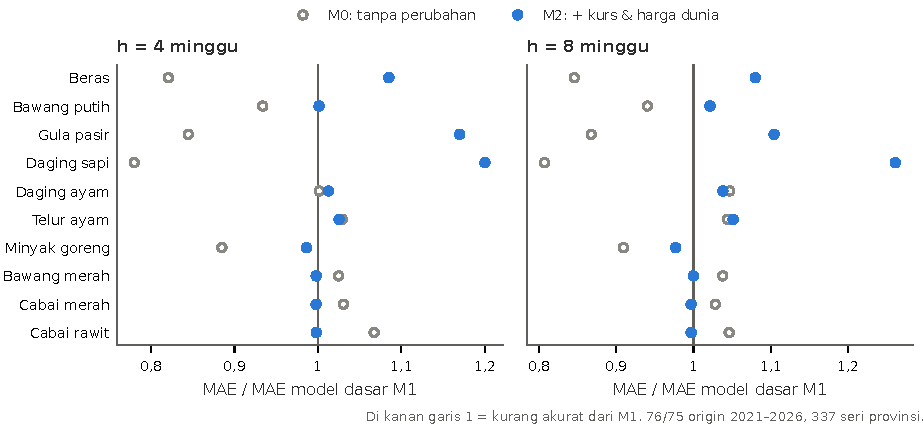
\includegraphics[width=\textwidth]{figures/prediksi_mae.pdf}
\caption{Rasio MAE per komoditas terhadap model dasar M1 untuk M2 (dengan fitur kurs dan harga dunia) dan M0 (tanpa perubahan).
Sumber: artefak \texttt{forecast\_eval}.}
\label{fig:prediksi}
\end{figure}

H5 tidak didukung. Pada origin dengan pergerakan kurs besar, rasio M2/M1 pada $h=8$ adalah 1,11 untuk jalur impor langsung ($p$ satu
sisi 0,93) dan 1,12 untuk input impor (0,86), dengan $p$ Holm 1,0. Hanya ada 8 origin seperti itu (7 tidak tumpang tindih), sehingga
daya ujinya rendah. Pada studi kasus 2026, rasio M2/M1 adalah 1,005 pada $h=4$ (10 origin) dan 1,004 pada $h=8$ (9 origin). Untuk
komoditas yang harganya diatur atau kaku, model tanpa perubahan lebih akurat daripada M1 pada $h=4$: daging sapi 0,78, beras 0,82,
gula 0,85, minyak goreng 0,89, dan bawang putih 0,93.

\subsection{Eksplorasi E2: rezim HET/HAP}

Pembagian periode menurut tanggal penetapan HET/HAP menghasilkan 145 sel (10 komoditas, 3–6 rezim, $h$ 4, 8, 12, terhadap kurs dan
harga dunia). Sebanyak 15 sel memiliki interval terkalibrasi yang tidak memuat nol, tetapi $q$ BH minimum 0,145, sehingga tidak ada
perbedaan antarrezim yang tahan koreksi multiplisitas. Pola terkuat yang kami catat ada pada bawang putih di rezim Perbadan 12/2024,
dengan $\beta_e(8) = 3,74$ \ci{1,83}{5,65} dalam 98 minggu, padahal sampel penuh memberi $-0,68$.

\subsection{Ketahanan dan validasi}

Estimasi utama berada di dalam interval cek pada 366 dari 382 sel Tier 1 (Tabel~\ref{tab:tier}). Dari 16 pengecualian, 10 ada pada
gula dan minyak goreng karena besarannya berbeda antar sub-periode, dan 3 pada daging ayam. Pada Tier 2, 191 dari 193 sel cocok.
Dua pengecualian Tier 2 bertanda sama dengan estimasi utama. Minyak goreng curah ternyata lebih peka terhadap harga sawit dunia,
dengan $\omega(8) = 0,36$ \ci{0,26}{0,45} dibanding 0,21 untuk minyak goreng kemasan. Implikasi proyeksi lokal berada di dalam
interval studi peristiwa pada 26 dari 30 sel, tetapi hanya 2 dari 30 interval studi peristiwa yang tidak memuat nol dan kesamaan
tanda antar episode hanya 0,51. Karena itu kecocokan ini lemah sebagai validasi.

\begin{table}[!htbp]
\centering\small
\caption{Pemeriksaan ketahanan: jumlah sel yang estimasi utamanya berada di dalam interval cek. Sumber: artefak \texttt{robustness}.}
\label{tab:tier}
\begin{tabularx}{\textwidth}{@{}>{\RaggedRight}X r@{\qquad}>{\RaggedRight}X r@{}}
\toprule
Cek Tier 1 & Sel cocok & Cek Tier 2 & Sel cocok \\
\midrule
Jumlah lag 2/4/8 & 96/96 & Varian PIHPS lain, komposit pakan lain & 94/96 \\
Dekomposisi kurs (dolar global, spesifik rupiah) & 78/78 & Harga mingguan dari observasi terakhir & 48/48 \\
Frekuensi bulanan & 47/48 & Panel Harga Bapanas bulanan & 42/42 \\
$h$ 8 dibanding 12 & 15/16 & Keterpencilan alternatif & 6/6 \\
Tanpa Mar–Jun 2020 dan bulan Brent ekstrem & 45/48 & Ordinal jalur eksposur & 1/1 \\
Sub-periode sebelum/sesudah 2021-04-05 & 85/96 & & \\
\bottomrule
\end{tabularx}
\end{table}

\subsection{Eksplorasi pasca-praregistrasi (tingkat 3)}

Karena kurs tidak membantu prediksi, kami bertanya informasi apa yang membantu TPID memprioritaskan pemantauan. Analisis ini
tidak menguji hipotesis. Seleksi model dan fitur dilakukan pada origin pengembangan (target sampai 2023), dan periode 2024 ke atas
dibuka untuk beberapa perbandingan. Karena periode itu dipakai berulang, kami mengoreksi sepuluh perbandingan sekaligus dengan Holm.
Semua varian yang pernah diuji, termasuk yang gagal, tercatat dalam registri eksperimen sebanyak 195 baris.

TimesFM 3.0 tanpa pelatihan pada data kami \citep{das2024,google2026} menurunkan MAE terhadap M1 menjadi 0,935 ($h=4$) dan 0,895
($h=8$), keduanya dengan DM $p<0,001$. Karena korpus pralatihnya tidak kami ketahui dan mungkin memuat deret harga pangan Indonesia,
keunggulan ini kami anggap batas atas. Klasifier arah berbasis dinamika harga (gradient boosting dengan fitur lag panjang, momentum,
volatilitas, musim, dan deviasi dari rerata bergerak serta provinsi lain) mencapai F1 makro 0,677 \ci{0,652}{0,698} pada $h=4$ dan
0,680 \ci{0,653}{0,706} pada $h=8$ untuk origin 2024 ke atas, di atas TimesFM sebesar 0,059 dan 0,053 ($p$ Holm 0,008). Kurs juga
tidak menambah akurasi pada keluarga model mana pun.

Daftar pantau dua komoditas per provinsi per minggu dari skor klasifier memuat kenaikan material (20\% perubahan terbesar
komoditas itu pada data latih) dengan presisi 0,18 \ci{0,13}{0,23} pada $h=4$ dan 0,16 \ci{0,11}{0,21} pada $h=8$. Aturan sederhana
terbaik hanya mencapai 0,085 dan 0,089, setara laju-dasar 0,088 dan 0,089, sehingga selisihnya 0,094 \ci{0,055}{0,132} dan 0,072
\ci{0,034}{0,115}. Daftar ini menangkap 41\% dan 36\% kenaikan material. Terhadap aturan ``pantau komoditas yang paling sering naik'',
keunggulannya terbukti pada $h=4$ (0,082; \ci{0,050}{0,120}) tetapi tidak pada $h=8$. Klasifier yang dilatih langsung pada target
kenaikan material mengurutkan risiko lebih baik pada $h=4$ (average precision 0,24 dibanding 0,19; selisih 0,045 \ci{0,017}{0,083}),
tetapi tidak terbukti pada $h=8$. Bukti out-of-sample yang bersih untuk tingkat ini hanya dapat datang dari validasi prospektif.
Prediksi untuk minggu yang belum terjadi sudah kami bekukan dan commit ke git sebelum target pertama tersedia (27 November 2026),
dengan evaluasi terjadwal 20 Desember 2026 dan 17 Januari 2027.

\subsection{Produk dan reproduksibilitas}

Hasil disajikan dalam aplikasi Streamlit yang hanya membaca artefak dan tidak melakukan estimasi saat dijalankan
(Gambar~\ref{fig:app}). Aplikasi ini memuat delapan halaman hasil, yaitu ringkasan, lini masa rupiah, respons harga, profil provinsi,
perbedaan antarprovinsi, faktor penjelas, prediksi, dan simulasi pelemahan rupiah, serta dua lampiran berisi data, metode, dan laporan
lengkap. Setiap grafik menampilkan rentang 95\% dan label asosiasi historis. Versi daringnya tersedia di
\url{https://kagami.streamlit.app}. Peta provinsi memakai geometri geoBoundaries \citep{runfola2020}.

\begin{figure}[!tbp]
\centering
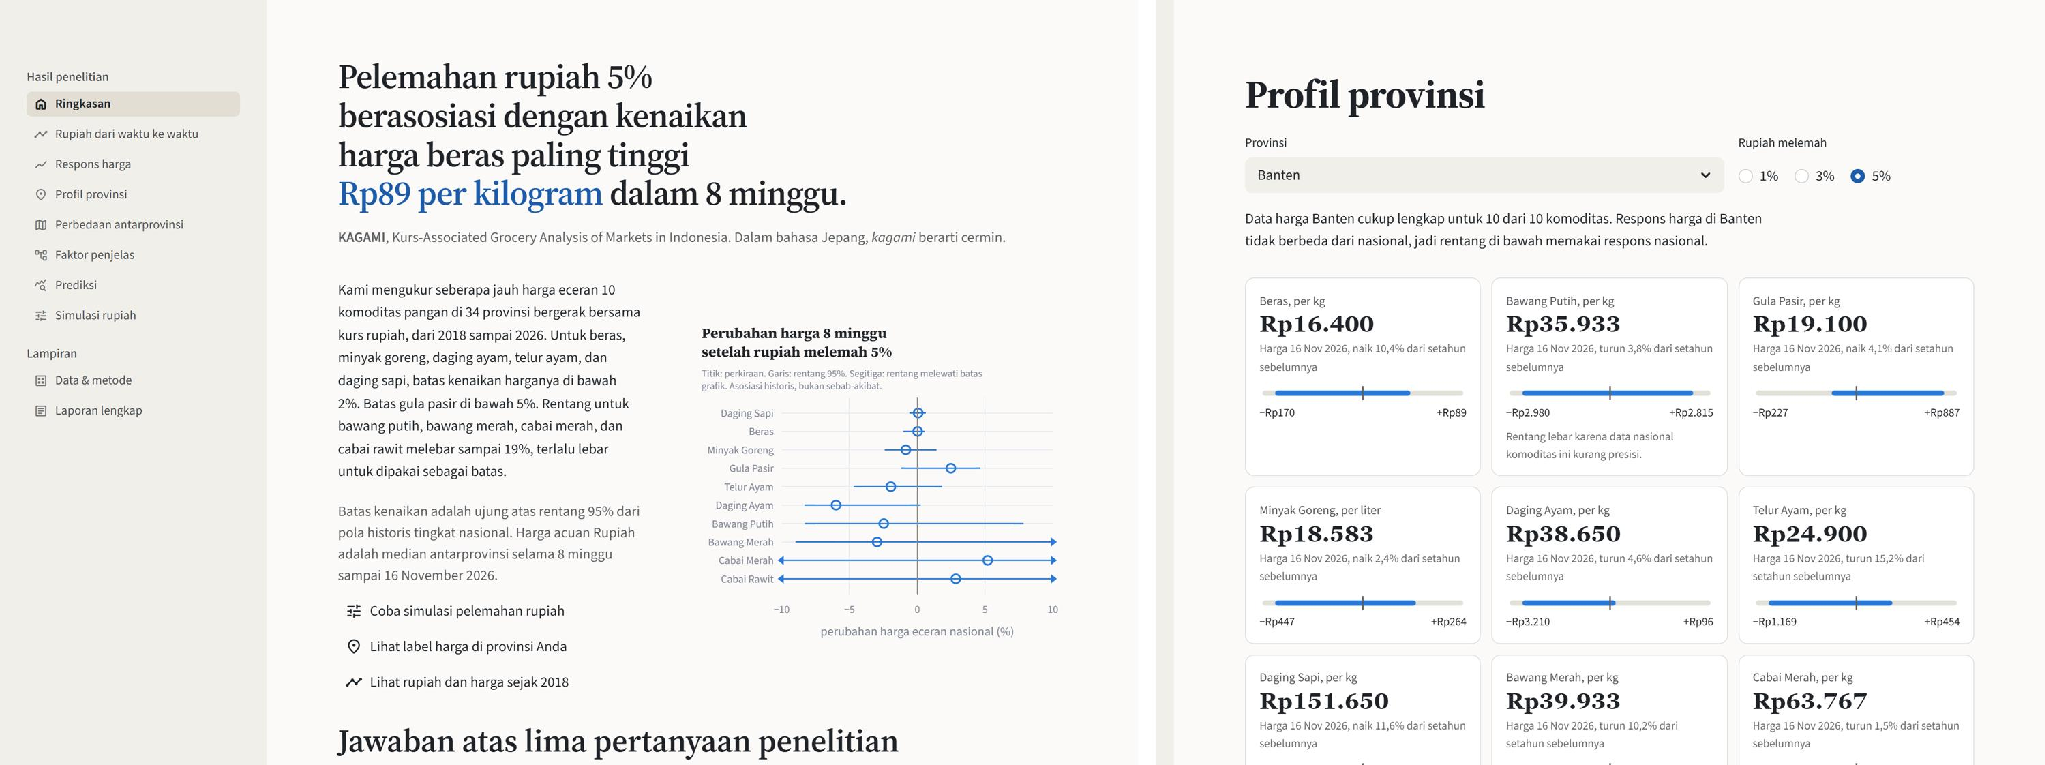
\includegraphics[width=\textwidth]{figures/app_layar.pdf}
\caption{Aplikasi KAGAMI. Kiri: halaman ringkasan dengan jawaban yang dihitung dari artefak dan grafik batas perubahan harga.
Kanan: profil provinsi berisi harga terkini dan rentang Rupiah untuk skenario pelemahan rupiah bagi setiap komoditas.}
\label{fig:app}
\end{figure}

Paket proyek berisi kode, konfigurasi, dataset turunan, seluruh artefak hasil, log eksekusi, dan aplikasi. Juri dapat mereproduksi
pada tiga tingkat. Tingkat A menjalankan aplikasi dari hasil (\texttt{python -m kagami app}). Tingkat B menjalankan semua tahap dari
dataset turunan yang dikirim (\texttt{python -m kagami all}, sekitar 1,9 jam di laptop). Tingkat C mengunduh ulang data mentah dari
sumber resmi. Gladi ulang dari folder bersih memastikan aplikasi berjalan dari isi paket, dan 428 tes otomatis lolos pada
28 November 2026. Run end-to-end penuh pada 24 November 2026 mereproduksi 35 artefak, 17 di antaranya identik byte demi byte dan
16 berselisih paling besar $3,5\times 10^{-11}$.

% ===========================================================================================================
\section{Analisis}

\subsection{Komoditas atau lokasi}
\label{sec:pemandu}

Dalam sampel 10 komoditas, titik estimasi respons nasional berbeda-beda antarkomoditas, dari $-1,67$ (daging ayam) sampai 1,37
(cabai merah) pada $h=8$, tetapi sebagian besar intervalnya memuat nol. Heterogenitas antarprovinsi di atas plasebo hanya terdeteksi
pada telur dan daging ayam, dan provinsi tidak membentuk kelompok. Kami tidak melakukan dekomposisi varians formal, jadi hasil ini
belum membuktikan bahwa komoditas lebih menentukan daripada lokasi. Yang kami amati adalah variasi titik estimasi antarkomoditas dan
heterogenitas provinsi yang jarang terdeteksi, dengan daya deteksi yang berbeda antarkomoditas. Bagi TPID, implikasinya praktis:
profil nasional per komoditas adalah titik awal yang wajar di semua provinsi, kecuali untuk telur dan daging ayam.

\subsection{Mengapa respons terhadap kurs kecil}

Ada tiga pola yang konsisten dengan hasil ini. Pertama, beras, daging sapi, gula, dan minyak goreng adalah komoditas yang harganya
diatur HET atau HAP dan didominasi rangkaian harga identik (85–92\% minggu). Minggu tanpa perubahan membatasi respons yang dapat
teramati, dan untuk beras serta daging sapi respons yang tersisa sangat kecil. Pola ini juga sejalan dengan temuan bahwa biaya distribusi lokal dan penyesuaian
harga yang jarang meredam penerusan kurs \citep{burstein2003,campa2010,gopinath2010}. Kedua, untuk minyak goreng, yang berasosiasi
dengan harga eceran adalah harga sawit dunia dalam rupiah, bukan kurs itu sendiri. Hal ini konsisten dengan transmisi lewat paritas
ekspor komoditas, dan minyak goreng curah yang tidak bermerek lebih peka daripada kemasan. Ketiga, tanda negatif daging ayam belum
dapat kami jelaskan. Asosiasi itu melemah tanpa periode Maret–Juni 2020, sehingga sebagian mungkin berasal dari guncangan permintaan
dan pasokan yang kebetulan bersamaan dengan episode depresiasi. Kami tidak menafsirkannya sebagai hubungan sebab-akibat.

\subsection{Makna bagi TPID: batas atas dalam Rupiah}

Hasil nol tetap berguna bila diterjemahkan ke batas atas dalam Rupiah (Tabel~\ref{tab:rupiah} dan Gambar~\ref{fig:batas}). Rumusnya
adalah perubahan $= \exp\!\big(PT(8)\cdot \ln 1,05\big) - 1$ dengan $PT(8)$ nasional dan interval resmi, dan harga acuan adalah median
antarprovinsi dari rerata harga teramati 8 minggu sampai 2026-11-16. Untuk enam komoditas, kenaikan harga yang berasosiasi dengan
pelemahan rupiah 5\% dan melebihi batas atas interval dapat dikesampingkan. Batas atas itu +0,25\% sampai +4,65\%, atau +Rp89 sampai
+Rp938 per kilogram atau liter. Intervalnya tidak simetris.

\begin{table}[!htbp]
\centering\footnotesize
\caption{Perubahan harga eceran nasional 8 minggu untuk skenario rupiah melemah 5\%, dengan interval resmi. Skenario bersyarat
dari pola historis, bukan ramalan. Sumber: artefak \texttt{profiles} dan \texttt{panel\_weekly}.}
\label{tab:rupiah}
\begin{tabular*}{\textwidth}{@{\extracolsep{\fill}}l r c c c@{}}
\toprule
Komoditas & Harga acuan (Rp) & Perubahan harga & Dalam Rupiah & Batas berguna \\
\midrule
Beras (kg) & 16.392 & +0,02\% \ci{−1,04}{+0,55\%} & +3 \ci{−170}{+89} & ya \\
Daging sapi (kg) & 150.525 & +0,06\% \ci{−0,58}{+0,62\%} & +91 \ci{−872}{+938} & ya \\
Daging ayam (kg) & 38.260 & −5,99\% \ci{−8,31}{+0,25\%} & −2.294 \ci{−3.178}{+95} & ya \\
Minyak goreng (liter) & 23.140 & −0,85\% \ci{−2,41}{+1,42\%} & −196 \ci{−557}{+328} & ya \\
Telur ayam (kg) & 29.462 & −1,95\% \ci{−4,69}{+1,82\%} & −575 \ci{−1.383}{+537} & ya \\
Gula pasir (kg) & 19.372 & +2,47\% \ci{−1,19}{+4,65\%} & +479 \ci{−231}{+900} & sedang \\
Bawang putih (kg) & 36.784 & −2,47\% \ci{−8,29}{+7,83\%} & −910 \ci{−3.051}{+2.881} & tidak \\
Bawang merah (kg) & 37.942 & −2,97\% \ci{−8,97}{+11,95\%} & −1.125 \ci{−3.404}{+4.532} & tidak \\
Cabai merah (kg) & 79.642 & +5,19\% \ci{−10,22}{+18,91\%} & +4.133 \ci{−8.143}{+15.061} & tidak \\
Cabai rawit (kg) & 89.660 & +2,84\% \ci{−18,44}{+16,09\%} & +2.545 \ci{−16.532}{+14.424} & tidak \\
\bottomrule
\end{tabular*}
\end{table}

\begin{figure}[!tbp]
\centering
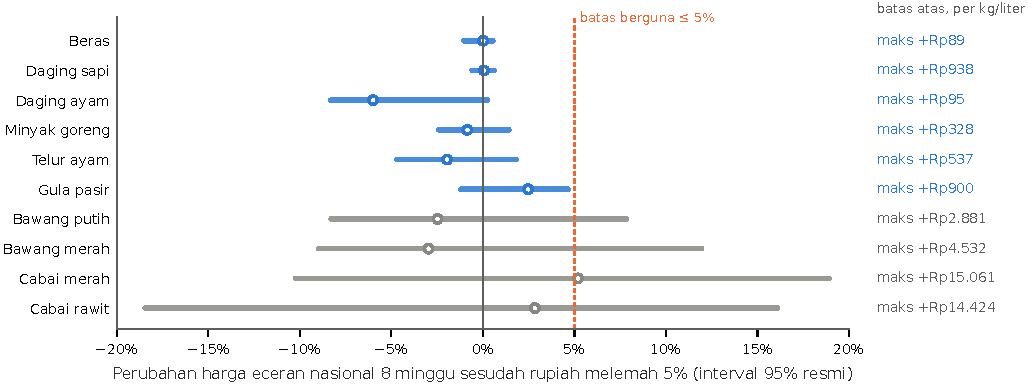
\includegraphics[width=\textwidth]{figures/batas_rupiah.pdf}
\caption{Perubahan harga eceran nasional 8 minggu sesudah rupiah melemah 5\%, dengan interval resmi. Biru = batas atas di bawah 5\%,
sehingga berguna sebagai batas. Di kanan: batas atas dalam Rupiah per kilogram atau liter. Sumber: artefak \texttt{profiles} dan
\texttt{panel\_weekly}.}
\label{fig:batas}
\end{figure}

Contoh pemakaiannya sebagai berikut. Misalkan harga beras naik Rp500 per kilogram dalam 8 minggu setelah rupiah melemah 5\%. Bagian
yang konsisten dengan asosiasi kurs historis paling banyak sekitar Rp89 per kilogram. Sisa kenaikan perlu ditelusuri ke faktor lain,
seperti pasokan, musim, kebijakan, atau faktor yang tidak teramati. Hasil nol tidak mengidentifikasi faktor itu, hanya mengarahkan
penelusuran. Untuk minyak goreng, kenaikan harga sawit dunia dalam rupiah sebesar 10\% berasosiasi dengan kenaikan harga minyak
goreng kemasan 1,5\% \ci{0,2}{2,7\%} pada $h=4$, atau sekitar Rp350 per liter \ci{Rp37}{Rp620}. Jadi TPID lebih tepat memantau harga
sawit dunia dalam rupiah daripada kurs itu sendiri.

Daftar pantau eksploratif dapat membantu memprioritaskan pemeriksaan data harga dan stok. Kira-kira satu dari enam komoditas yang
ditandai benar-benar naik material, sehingga daftar ini belum layak dipakai untuk intervensi otomatis. Sekitar 57\% tanda jatuh pada
beras, gula, minyak goreng, dan daging sapi, yang ambang material statistiknya hanya 1,4–2,7\%. Ambang kebijakan TPID mungkin
berbeda dan perlu ditetapkan bersama pengguna.

\subsection{Kualitas inferensi}
\label{sec:inferensi}

Sesudah praregistrasi kami menemukan dua masalah inferensi dengan arah berlawanan. Bootstrap blok 13 minggu lebih pendek dari jendela
proyeksi lokal ($h+6$ minggu), sehingga rerata replikasi hanya 0,57, 0,35, dan 0,35 kali estimasi (median, pada $h$ 4, 8, dan 12).
Akibatnya interval resmi cenderung terlalu lebar. Sebaliknya, galat baku berkelompok per minggu terlalu sempit. Di bawah plasebo,
$|t|>1,96$ terjadi pada 8,8\% replikasi per sel nasional (maksimum 17,6\%), padahal seharusnya 5\%.

Sebagai analisis kepekaan (tingkat 2), kami memakai distribusi statistik $t$ dari plasebo sebagai null, dengan interval
$\hat\beta \pm \mathrm{crit}\cdot SE$ dan $\mathrm{crit} = \max(1,96;\ \text{kuantil plasebo})$. Ukurannya kami uji dengan
memperlakukan setiap replikasi plasebo sebagai data asli (Tabel~\ref{tab:kalibrasi}). Kalibrasi tidak memilih metode yang paling
banyak memberi hasil signifikan. Ambangnya lebih ketat daripada 1,96 pada 41 dari 48 sel (median 2,28), dan positif palsunya 4,4\%.
Dua klaim hanya bergantung pada tingkat ini, yaitu daging ayam $\beta_e(8)$ ($q$ 0,058) dan minyak goreng $\omega(8)$ ($q$ 0,024).
Klaim lain didukung interval resmi.

\begin{table}[!htbp]
\centering\small
\caption{Uji ukuran inferensi pada 48 sel nasional ($\beta_e$ dan $\omega$, $h$ 4, 8, 12) di bawah null plasebo.}
\label{tab:kalibrasi}
\begin{tabularx}{\textwidth}{@{}>{\RaggedRight}X *{4}{>{\centering\arraybackslash}p{2.45cm}}@{}}
\toprule
Metode & Positif palsu per sel & Replikasi null dengan $\ge 1$ temuan BH & Data asli: sel tidak memuat nol & Data asli: temuan BH \\
\midrule
$\pm 1,96\cdot SE$ berkelompok per minggu & 8,8\% (maks 17,6\%) & 17,1\% & 9 & 5 \\
Terkalibrasi plasebo & 4,4\% (maks 4,8\%) & 0,5\% & 7 & 4 \\
Resmi praregistrasi & tidak dapat diuji & -- & 3 & -- \\
\bottomrule
\end{tabularx}
\end{table}

\subsection{Ancaman validitas}

Evaluasi prediktif bersifat pseudo-real-time. Jendela revisi data PIHPS belum dapat kami pastikan, sehingga waktu keputusan Task 4
kami tetapkan secara konservatif pada Minggu pukul 00.00 sesudah minggu origin. Harga dunia memakai rilis Pink Sheet 3 November 2026
yang memuat revisi historis. Proksi provinsi terbatas. Jarak garis lurus tidak mencakup biaya logistik, kecukupan produksi hanya
mencakup beras, dan jumlah kota sampel tidak sama dengan tingkat integrasi pasar. Rasio impor memiliki mutu yang berbeda
antarkomoditas. Kerangka 34 provinsi lama dipertahankan agar seri tetap sebanding. Pada eksplorasi Task 4, periode uji dipakai
berulang dan TimesFM mungkin pernah melihat data uji. Kebutuhan pengguna belum divalidasi, sehingga belum ada bukti bahwa daftar
pantau memperbaiki keputusan operasional.

% ===========================================================================================================
\section{Kesimpulan dan Saran}

\subsection{Kesimpulan}

Kami membangun dataset turunan harga pangan eceran mingguan 10 komoditas di 34 provinsi yang terintegrasi dengan kurs, harga dunia
dalam rupiah, dan regulasi, lalu menguji hipotesis yang dibekukan sebelum hasil dilihat. Kesimpulan utamanya sebagai berikut.
\begin{enumerate}
\item Di antara 10 komoditas yang diamati, respons nasional harga eceran terhadap kurs sebagian besar tidak terdeteksi. Asosiasi
yang paling konsisten ada pada minyak goreng dan harga sawit dunia dalam rupiah.
\item Heterogenitas antarprovinsi di atas plasebo hanya terdeteksi pada telur dan daging ayam (yang terakhir rapuh), dan provinsi
tidak membentuk kelompok. Struktur 2–3 kelompok seimbang dengan selisih respons minimal 0,2 per fitur akan terdeteksi.
\item Respons saat rupiah melemah tidak terbukti berbeda dari saat menguat. Uji konfirmatori untuk beras dan daging sapi tidak
menolak hipotesis nol.
\item Rasio impor langsung tidak berasosiasi monoton dengan penerusan kurs, dan keterpencilan provinsi tidak berasosiasi dengan
respons 4 minggu.
\item Fitur kurs dan harga dunia tidak menurunkan galat prediksi 4 dan 8 minggu. Model dengan fitur kurs sedikit lebih buruk,
sehingga H5 tidak didukung.
\item Hasil nol memberi batas atas dalam Rupiah yang dapat dipakai TPID untuk enam komoditas: kenaikan harga 8 minggu yang konsisten
dengan pelemahan rupiah 5\% paling tinggi +Rp89 sampai +Rp938 per kilogram atau liter.
\end{enumerate}

\subsection{Saran}

Bagi TPID, kami menyarankan empat langkah. Batas atas Rupiah dapat dipakai untuk memisahkan bagian kenaikan harga yang konsisten
dengan pelemahan rupiah dari bagian yang perlu ditelusuri ke faktor lain. Untuk minyak goreng, harga sawit dunia dalam rupiah lebih
layak dipantau daripada kurs. Profil nasional dapat menjadi titik awal di semua provinsi, kecuali untuk telur dan daging ayam.
Daftar pantau sebaiknya baru dipakai sesudah ambang kebijakan dan kapasitas pemantauan disepakati bersama pengguna.

Bagi penelitian lanjutan, kebutuhan TPID perlu divalidasi lewat wawancara dengan panduan yang sudah kami siapkan. Data pasokan,
seperti stok mingguan dan proyeksi neraca pangan, perlu diminta secara resmi karena belum tersedia untuk publik. Jendela revisi dan
vintage data PIHPS perlu dipastikan. Data tingkat kabupaten dan kota dapat memperluas analisis bila izinnya tersedia. Validasi
prospektif perlu diselesaikan pada jadwalnya, dan dekomposisi varians formal antara komoditas dan provinsi serta bootstrap dengan blok
yang lebih panjang dari jendela estimasi perlu diuji.

% ===========================================================================================================
\clearpage
\section*{Daftar Pustaka}
\addcontentsline{toc}{section}{Daftar Pustaka}
\begingroup\small
\begin{list}{}{\leftmargin=1.6em \itemindent=-1.6em \itemsep=1.5pt \parsep=0pt \topsep=2pt}
\refitem{aginta2022} Aginta, H., \& Someya, M. (2022). Regional economic structure and heterogeneous effects of monetary policy:
Evidence from Indonesian provinces. \textit{Journal of Economic Structures, 11}, Article 1. \url{https://doi.org/10.1186/s40008-021-00260-6}
\refitem{almuzara2024} Almuzara, M., \& Sancibrián, V. (2024). \textit{Micro responses to macro shocks} (Staff Report No. 1090).
Federal Reserve Bank of New York. \url{https://doi.org/10.59576/sr.1090}
\refitem{amatullah2025} Amatullah, F. F., Ilmani, E. A., Fitrianto, A., Erfiani, E., \& Jumansyah, L. M. R. D. (2025). Clustering time
series forecasting model for grouping provinces in Indonesia based on granulated sugar prices. \textit{Journal of Applied Informatics
and Computing, 9}(1), 121–130. \url{https://doi.org/10.30871/jaic.v9i1.8840}
\refitem{amiti2014} Amiti, M., Itskhoki, O., \& Konings, J. (2014). Importers, exporters, and exchange rate disconnect.
\textit{American Economic Review, 104}(7), 1942–1978. \url{https://doi.org/10.1257/aer.104.7.1942}
\refitem{apaitan2024} Apaitan, T., Manopimoke, P., Nookhwun, N., \& Pattararangrong, J. (2024). Heterogeneity in exchange rate
pass-through to import prices in Thailand: Evidence from micro data. \textit{Journal of International Money and Finance, 149},
103196. \url{https://doi.org/10.1016/j.jimonfin.2024.103196}
\refitem{arintoko2024} Arintoko, A., Badriah, L. S., \& Kadarwati, N. (2024). The asymmetric effects of global energy and food prices,
exchange rate dynamics, and monetary policy conduct on inflation in Indonesia. \textit{Ekonomika, 103}(2), 66–89.
\url{https://doi.org/10.15388/Ekon.2024.103.2.4}
\refitem{bapanas2026} Badan Pangan Nasional. (2026). \textit{Panel Harga Pangan}. Diakses November 2026, dari
\url{https://panelharga.badanpangan.go.id/}
\refitem{bps2026} Badan Pusat Statistik. (2026). \textit{Data ekspor impor}. Diakses November 2026, dari \url{https://www.bps.go.id/id/exim}
\refitem{bijisdor2026} Bank Indonesia. (2026a). \textit{Jakarta Interbank Spot Dollar Rate (JISDOR)}. Diakses November 2026, dari
\url{https://www.bi.go.id/id/statistik/informasi-kurs/jisdor/default.aspx}
\refitem{bipihps2026} Bank Indonesia. (2026b). \textit{Pusat Informasi Harga Pangan Strategis Nasional (PIHPS Nasional)}. Diakses
November 2026, dari \url{https://www.bi.go.id/hargapangan}
\refitem{bh1995} Benjamini, Y., \& Hochberg, Y. (1995). Controlling the false discovery rate: A practical and powerful approach to
multiple testing. \textit{Journal of the Royal Statistical Society: Series B (Methodological), 57}(1), 289–300.
\url{https://doi.org/10.1111/j.2517-6161.1995.tb02031.x}
\refitem{burstein2003} Burstein, A. T., Neves, J. C., \& Rebelo, S. (2003). Distribution costs and real exchange rate dynamics during
exchange-rate-based stabilizations. \textit{Journal of Monetary Economics, 50}(6), 1189–1214.
\url{https://doi.org/10.1016/S0304-3932(03)00075-8}
\refitem{campa2010} Campa, J. M., \& Goldberg, L. S. (2010). The sensitivity of the CPI to exchange rates: Distribution margins,
imported inputs, and trade exposure. \textit{Review of Economics and Statistics, 92}(2), 392–407.
\url{https://doi.org/10.1162/rest.2010.11459}
\refitem{chen2023} Chen, S.-A., Li, C.-L., Yoder, N., Arik, S. O., \& Pfister, T. (2023). TSMixer: An all-MLP architecture for time
series forecasting. \textit{Transactions on Machine Learning Research}. \url{https://arxiv.org/abs/2303.06053}
\refitem{clark2026} Clark, T., \& Huber, F. (2026). \textit{Clustered local projections for short and ultra-short time series: A
hierarchical Bayesian framework} (arXiv:2608.04631). \url{https://arxiv.org/abs/2608.04631}
\refitem{das2024} Das, A., Kong, W., Sen, R., \& Zhou, Y. (2024). \textit{A decoder-only foundation model for time-series
forecasting} (arXiv:2310.10688). \url{https://arxiv.org/abs/2310.10688}
\refitem{dl1986} DerSimonian, R., \& Laird, N. (1986). Meta-analysis in clinical trials. \textit{Controlled Clinical Trials, 7}(3),
177–188. \url{https://doi.org/10.1016/0197-2456(86)90046-2}
\refitem{dm1995} Diebold, F. X., \& Mariano, R. S. (1995). Comparing predictive accuracy. \textit{Journal of Business \& Economic
Statistics, 13}(3), 253–263. \url{https://doi.org/10.1080/07350015.1995.10524599}
\refitem{fao2026} FAO. (2026). \textit{FAOSTAT: Supply Utilization Accounts} (CC BY 4.0). Diakses November 2026, dari
\url{https://www.fao.org/faostat/}
\refitem{fred2026} Federal Reserve Bank of St.\ Louis. (2026). \textit{FRED: Brent crude oil prices (DCOILBRENTEU) dan Nominal broad
U.S. dollar index (DTWEXBGS)}. Diakses November 2026, dari \url{https://fred.stlouisfed.org/}
\refitem{friedman2001} Friedman, J. H. (2001). Greedy function approximation: A gradient boosting machine. \textit{The Annals of
Statistics, 29}(5), 1189–1232. \url{https://doi.org/10.1214/aos/1013203451}
\refitem{gebru2021} Gebru, T., Morgenstern, J., Vecchione, B., Vaughan, J. W., Wallach, H., Daumé III, H., \& Crawford, K. (2021).
Datasheets for datasets. \textit{Communications of the ACM, 64}(12), 86–92. \url{https://doi.org/10.1145/3458723}
\refitem{gopinath2020} Gopinath, G., Boz, E., Casas, C., Díez, F. J., Gourinchas, P.-O., \& Plagborg-Møller, M. (2020). Dominant
currency paradigm. \textit{American Economic Review, 110}(3), 677–719. \url{https://doi.org/10.1257/aer.20171201}
\refitem{gopinath2010} Gopinath, G., \& Itskhoki, O. (2010). Frequency of price adjustment and pass-through. \textit{Quarterly Journal
of Economics, 125}(2), 675–727. \url{https://doi.org/10.1162/qjec.2010.125.2.675}
\refitem{google2026} Google Research. (2026). \textit{TimesFM 3.0} (google/timesfm-3.0-pytorch) [Model deret waktu]. Hugging Face.
\url{https://huggingface.co/google/timesfm-3.0-pytorch}
\refitem{hln1997} Harvey, D., Leybourne, S., \& Newbold, P. (1997). Testing the equality of prediction mean squared errors.
\textit{International Journal of Forecasting, 13}(2), 281–291. \url{https://doi.org/10.1016/S0169-2070(96)00719-4}
\refitem{hennig2007} Hennig, C. (2007). Cluster-wise assessment of cluster stability. \textit{Computational Statistics \& Data
Analysis, 52}(1), 258–271. \url{https://doi.org/10.1016/j.csda.2006.11.025}
\refitem{hoerl1970} Hoerl, A. E., \& Kennard, R. W. (1970). Ridge regression: Biased estimation for nonorthogonal problems.
\textit{Technometrics, 12}(1), 55–67. \url{https://doi.org/10.1080/00401706.1970.10488634}
\refitem{holm1979} Holm, S. (1979). A simple sequentially rejective multiple test procedure. \textit{Scandinavian Journal of
Statistics, 6}(2), 65–70. \url{https://www.jstor.org/stable/4615733}
\refitem{hubert1985} Hubert, L., \& Arabie, P. (1985). Comparing partitions. \textit{Journal of Classification, 2}(1), 193–218.
\url{https://doi.org/10.1007/BF01908075}
\refitem{ibrahim2025} Ibrahim, M., \& Nghiem, X.-H. (2025). Commodity prices and inflation in Indonesia: Does the pass-through really
matter? \textit{Australian Economic Papers, 65}(2), 149–163. \url{https://doi.org/10.1111/1467-8454.70018}
\refitem{jorda2005} Jordà, Ò. (2005). Estimation and inference of impulse responses by local projections. \textit{American Economic
Review, 95}(1), 161–182. \url{https://doi.org/10.1257/0002828053828518}
\refitem{kohlscheen2026} Kohlscheen, E., \& Mehrotra, A. (2026). \textit{What drives exchange rate pass-throughs? Evidence from a
non-parametric method} (BIS Working Papers No. 1371). Bank for International Settlements. \url{https://www.bis.org/publ/work1371.htm}
\refitem{kunsch1989} Künsch, H. R. (1989). The jackknife and the bootstrap for general stationary observations. \textit{The Annals of
Statistics, 17}(3), 1217–1241. \url{https://doi.org/10.1214/aos/1176347265}
\refitem{montiel2021} Montiel Olea, J. L., \& Plagborg-Møller, M. (2021). Local projection inference is simpler and more robust than
you think. \textit{Econometrica, 89}(4), 1789–1823. \url{https://doi.org/10.3982/ECTA18756}
\refitem{nie2023} Nie, Y., Nguyen, N. H., Sinthong, P., \& Kalagnanam, J. (2023). \textit{A time series is worth 64 words: Long-term
forecasting with transformers} (arXiv:2211.14730). \url{https://arxiv.org/abs/2211.14730}
\refitem{nosek2018} Nosek, B. A., Ebersole, C. R., DeHaven, A. C., \& Mellor, D. T. (2018). The preregistration revolution.
\textit{Proceedings of the National Academy of Sciences, 115}(11), 2600–2606. \url{https://doi.org/10.1073/pnas.1708274114}
\refitem{pedregosa2011} Pedregosa, F., Varoquaux, G., Gramfort, A., Michel, V., Thirion, B., Grisel, O., Blondel, M., Prettenhofer,
P., Weiss, R., Dubourg, V., Vanderplas, J., Passos, A., Cournapeau, D., Brucher, M., Perrot, M., \& Duchesnay, É. (2011).
Scikit-learn: Machine learning in Python. \textit{Journal of Machine Learning Research, 12}, 2825–2830.
\url{https://jmlr.org/papers/v12/pedregosa11a.html}
\refitem{persada2026} Persada, R., Subagyo, \& Wibowo, B. S. (2026). Regional heterogeneity in rice prices in Indonesia: A
province-level panel study of surplus and deficit areas. \textit{Frontiers in Sustainable Food Systems, 10}, 1844670.
\url{https://doi.org/10.3389/fsufs.2026.1844670}
\refitem{plagborg2021} Plagborg-Møller, M., \& Wolf, C. K. (2021). Local projections and VARs estimate the same impulse responses.
\textit{Econometrica, 89}(2), 955–980. \url{https://doi.org/10.3982/ECTA17813}
\refitem{pustejovsky2018} Pustejovsky, J. E., \& Tipton, E. (2018). Small-sample methods for cluster-robust variance estimation and
hypothesis testing in fixed effects models. \textit{Journal of Business \& Economic Statistics, 36}(4), 672–683.
\url{https://doi.org/10.1080/07350015.2016.1247004}
\refitem{rahkmawati2023} Rahkmawati, Y., \& Annisa, S. (2023). Clustering time series using dynamic time warping distance in
provinces in Indonesia based on rice prices. \textit{TIERS Information Technology Journal, 4}(2), 115–121.
\url{https://doi.org/10.38043/tiers.v4i2.5081}
\refitem{rousseeuw1987} Rousseeuw, P. J. (1987). Silhouettes: A graphical aid to the interpretation and validation of cluster
analysis. \textit{Journal of Computational and Applied Mathematics, 20}, 53–65. \url{https://doi.org/10.1016/0377-0427(87)90125-7}
\refitem{runfola2020} Runfola, D., Anderson, A., Baier, H., Crittenden, M., Dowker, E., Fuhrig, S., Goodman, S., Grimsley, G.,
Layko, R., Melville, G., Mulder, M., Oberman, R., Panganiban, J., Peck, A., Seitz, L., Shea, S., Slevin, H., Youngerman, R., \&
Hobbs, L. (2020). geoBoundaries: A global database of political administrative boundaries. \textit{PLOS ONE, 15}(4), e0231866.
\url{https://doi.org/10.1371/journal.pone.0231866}
\refitem{saputra2026} Saputra, M. J., Rahkmawati, Y., Annisa, S., \& Yolanda, A. M. (2026). Ensemble boosting models for forecasting
rice prices in Indonesia. \textit{Jurnal Aplikasi Statistika \& Komputasi Statistik, 18}(1), 115–129.
\url{https://doi.org/10.34123/jurnalasks.v18i1.973}
\refitem{schroer2021} Schröer, C., Kruse, F., \& Gómez, J. M. (2021). A systematic literature review on applying CRISP-DM process
model. \textit{Procedia Computer Science, 181}, 526–534. \url{https://doi.org/10.1016/j.procs.2021.01.199}
\refitem{solorzano2023} Solórzano, D. (2023). Heterogeneous exchange rate pass-through in Mexico: What drives it? \textit{Latin
American Journal of Central Banking, 4}(4), 100100. \url{https://doi.org/10.1016/j.latcb.2023.100100}
\refitem{suarsih2016} Suarsih, S., Achsani, N. A., \& Nuryartono, N. (2016). Dampak perubahan nilai tukar terhadap indeks harga
konsumen bahan makanan di Indonesia. \textit{Jurnal Ekonomi dan Pembangunan Indonesia, 17}(1), 1–14.
\url{https://doi.org/10.21002/jepi.v17i1.548}
\refitem{sumertajaya2024} Sumertajaya, I. M., Rohaeti, E., Fitrianto, A., \& Ponco Adi, W. (2024). Development of food commodity
price forecasting model as an early warning system with a multivariate time series clustering. \textit{Sains Malaysiana, 53}(11),
3779–3789. \url{https://doi.org/10.17576/jsm-2024-5311-20}
\refitem{un2015} United Nations General Assembly. (2015). \textit{Transforming our world: The 2030 Agenda for Sustainable Development}
(A/RES/70/1). \url{https://undocs.org/A/RES/70/1}
\refitem{unuvar2026} Unuvar, F. I. (2026). Threshold effects in exchange rate pass-through to food prices in emerging market
economies. \textit{Frontiers in Sustainable Food Systems, 10}, 1960606. \url{https://doi.org/10.3389/fsufs.2026.1960606}
\refitem{varela2013} Varela, G., Aldaz-Carroll, E., \& Iacovone, L. (2013). Determinants of market integration and price transmission
in Indonesia. \textit{Journal of Southeast Asian Economies (ASEAN Economic Bulletin), 30}(1), 19–44. \url{https://doi.org/10.1355/ae30-1b}
\refitem{ward1963} Ward, J. H. (1963). Hierarchical grouping to optimize an objective function. \textit{Journal of the American
Statistical Association, 58}(301), 236–244. \url{https://doi.org/10.1080/01621459.1963.10500845}
\refitem{widarjono2023} Widarjono, A., Alam, M. M., Atmadji, E., Suseno, P., \& Artiani, L. E. (2023). The asymmetric exchange rate
pass-through to inflation in the selected ASEAN countries. \textit{Bulletin of Monetary Economics and Banking, 26}(1), 105–124.
\url{https://doi.org/10.59091/1410-8046.2047}
\refitem{worldbank2026} World Bank. (2026). \textit{Commodity price data (The Pink Sheet)}, rilis 3 November 2026 (CC BY 4.0). Diakses
November 2026, dari \url{https://www.worldbank.org/en/research/commodity-markets}
\end{list}
\endgroup

\end{document}
